\documentclass[utf8]{gradu3}
% Jos työ on kandidaatintutkielma eikä pro gradu, käytä ylläolevan asemesta
%\documentclass[utf8,bachelor]{gradu3}
% Jos kirjoitat englanniksi, käytä ylläolevan asemesta
%\documentclass[utf8,english]{gradu3}
% tai
%\documentclass[utf8,bachelor,english]{gradu3}

\usepackage{graphicx} % kuvien mukaan ottamista varten
\graphicspath{ {./kuvat/} }

\usepackage{amsmath} % hyödyllinen jos tekstisi sisältää matikkaa,
                     % ei pakollinen

\usepackage{booktabs} % hyvä kauniiden taulukoiden tekemiseen

% HUOM! Tämän tulee olla viimeinen \usepackage koko dokumentissa!
\usepackage[bookmarksopen,bookmarksnumbered,linktocpage]{hyperref}

\addbibresource{gradu.bib} % Lähdetietokannan tiedostonimi

\begin{document}

\title{Äänipalautetyökalun suunnittelu, toteutus ja evaluointi}
\translatedtitle{Design, implementation and evaluation of recorded audio feedback -tool}
\studyline{Ohjelmistotekniikka}
\avainsanat{%
  suunnittelututkimus, äänipalaute, työkalu, audio-ohjelmisto, palautemuoto, heuristiikat, oppimisympäristö
  }
\keywords{design science, recorded audio feedback, tool, audio-software, feedback form, heuristics, virtual learning environment}
\tiivistelma{%
Palaute on yksi merkittävimpiä yksittäisiä tekijöitä oppimisen kannalta, ja sen tulisi olla   ajankohtaista, ymmärrettävää ja oppilaan hyödynnettävissä.  Aänipalaute on todettu tehokkaaksi palautemuodoksi tekstimuotoisen palautteen ohella, ja sen suosio on kasvanut opetuskäytössä vuosien varrella. Se on muun muassa yksityiskohtaisempaa, ymmärrettävempää ja henkilökohtaisempaa, kuin tekstimuotoinen palaute, sekä suhtautuminen sen antamiseen ja vastaanottamiseen on yleisesti positiivista. Äänipalautteen antaminen koostuu palautteen nauhoittamisesta ja sen jakamisesta, jotka voidaan suorittaa usein eri tavoin. Tässä suunnittelutukimuksessa suunniteltiin ja toteutettiin äänipalautteen antamiseen suunnattu web-pohjainen työkalu, jota evaluoimalla selvitettiin, voidaanko äänipalautteen antamista helpottaa entisestään tai voidaanko suhtautumista sen antamiseen muuttaa. Työkalun suunnittelussa ja toteutuksessa hyödynnettiin Nielsenin heuristiikkoja sekä Gestaltin hahmolakeja, ja osa ratkaisuista päätettiin yhteistyössä äänipalautetta opetuksessaan hyödyntäneiden pro gradu -ohjaajien kanssa. Työkalun evaluointi suoritettiin kahdessa iteraatiossa, joista ensimmäiseen osallistui kaksi koehenkilöä. Ensimmäisen evaluoinnin pohjalta työkaluun tehtiin parannuksia ja lisäominaisuuksia, jonka jälkeen suoritettiin toinen evaluointi neljän koehenkilön toimesta. Tulosten perusteella voidaan sanoa, että...
}
\abstract{%
  ...
}

\author{Erkko Mäkinen}
\contactinformation{\texttt{erkko.e.makinen@student.jyu.fi}}
% jos useita tekijöitä, anna useampi \author-komento
\supervisor{Anneli Heimbürger ja Ville Isomöttönen}
% jos useita ohjaajia, anna useampi \supervisor-komento

%\type{Tietotekniikan pro gradu -tutkielma} % et tarvitse tätä riviä tutkielmassa!

\maketitle

%\begin{thetermlist}
%\item[RAF] Recorded audio feedback \parencite[ks.][]{using}. 
%\end{thetermlist}

\mainmatter

\chapter{Johdanto}

Palautteenanto on erittäin tärkeä osa opetusta, jotta opiskelijat tietäisivät missä asioissa he ovat suoriutuneet hyvin ja missä heillä olisi vielä kehittämisen varaa. Se voidaan suorittaa usein eri tavoin, ja siinä voidaan hyödyntää erilaisia palutemuotoja, joista kullakin on omat hyvät ja huonot puolensa. Äänipalautteen (engl. Recorded Audio Feedback, RAF) hyödyntäminen opetuskäytössä on yleistynyt lähivuosina, erityisesti verkko-oppimisen parissa, jossa suoraa kontaktia opettajaan tai muihin opiskelijoihin ei välttämättä ole lainkaan. Se on validi palautemuoto tekstimuotoisen palautteen ohella, etenkin kun opiskelu muuttuu vuosi vuodelta yhä teknologia-avusteisemmaksi, on tilanteeseen mukauduttava myös palautteenannon kannalta, jotta palaute olisi mahdollisimman tehokasta.

Tämän hetkisten tutkimusten perusteella voidaan sanoa, että äänipalaute koetaan yleisesti positiivisena sekä opettajien että oppilaiden keskuudessa. Äänipalautetta pystytään antamaan nopeasti, se on tekstimuotoista yksityiskohtaisempaa ja selkeämpää, sekä asiat voidaan käsitellä keskustelunomaisesti vaikeasti ymmärrettävän akateemisen kielen sijaan \parencite[][]{developing}. Lisäksi äänensävyllä voidaan korostaa ja helpottaa palautteen tulkitsemista ja palautteen kuuleminen lukemisen sijaan tuntuu henkilökohtaisemmalta, mikä vaikuttaa positiivisesti oppimiseen \parencite[][]{attitudes}. Äänipalaute toimii parhaiten täydentävänä tai vaihtoehtoisena palautemuotona tekstimuotoisen palautteen ohella, ja se soveltuu erityisesti kirjoitustehtäviin. Tarkkuutta vaativiin tehtäviin kuitenkin soveltuu paremmin tekstimuotoinen palaute \parencite[][]{academics}. Opiskelijoiden mukaan äänipalaute tukee oppimista parhaiten siten, että palautteen pääkohdat ovat kirjattu tekstimuotoisena sähköpostiin ja yksityiskohtaisemmat perustelut niitä koskien äänipalautteeseen \parencite[][]{using}.

Vaikka äänipalautteella on tutkittu olevan selkeitä etuja tekstimuotoiseen palautteeseen nähden, se asettaa tiettyjä teknisiä vaatimuksia sekä opettajille että oppilaille, jotka voivat johtaa jopa palautemuodon poissulkemiseen \parencite[][]{developing}. Äänipalautteen nauhoittaminen ja jakaminen voidaan suorittaa useilla eri työkaluilla ja alustoilla, mutta audio-ohjelmistot sisältävät yleensä paljon epäolennaisia toiminnallisuuksia, jotka voivat vaikeuttaa niiden oppimista ja käyttämistä. Toisaalta osa työkaluista taas mahdollistaa ainoastaan palautteen nauhoittamisen, jolloin virheen sattuessa nauhoitusprosessi on aloitettava alusta. Erilaiset alkukömpelyydestä johtuvat seikat voivat turhauttaa opettajaa, jonka seurauksena kokemus äänipalautteen antamisesta voi kärsiä \parencite[][]{versus}.

Tämän suunnittelututkimuksen tavoitteena on suunnitella, kehittää ja evaluoida äänipalautteen antamiseen tarkoitettu prototyyppi-työkalu, joka mahdollistaa äänileikkeiden nauhoittamisen ja editoimisen mahdollisimman helposti. Tutkimus suoritetaan kahdessa iteraatiossa, jotka molemmat koostuuvat työkalun suunnittelusta, kehittämisestä ja evaluoinnista. Evaluointi suoritetaan ensimmäisessä iteraatiossa kahden koehenkilön toimesta, ja toisessa iteraatiossa neljän koehenkilön toimesta. Koehenkilöillä on aiempaa kokemusta äänipalautteen antamista, joten he voivat verrata työkalun käyttöä aiempiin kokemuksiinsa. Tutkimuksen pääpaino on työkalun evaluoinnissa, jossa koehenkilöiden tulee käyttää äänipalautetyökalua autenttisessa tilanteessa, ja vastata lomakkeella esitettyihin kysymyksiin työkalua koskien. Tulosten perusteella pyritään vastaamaan kahteen tutkimuskysymykseen:

\begin{itemize}
  \item Helpottaako äänipalautetyökalu äänipalautteen antamista entuudestaan?
  \item Muuttaako äänipalautetyökalun käyttö suhtautimista äänipalautteen antamiseen?
\end{itemize}

Luvussa 1 käydään läpi tarkemmin suunnittelututkimuksen eri vaiheita, ja kuinka tutkimus kokonaisuudessaan toteutetaan. Luku 2 käsittelee palautteenantoa ja äänipalautetta yleisesti, äänipalautteen hyviä ja huonoja puolia sekä äänipalautteen antamista opettajan näkökulmasta. Luvussa 3 editetään äänipalautetyökalun tekniset toteutusratkaisut, suunnitteluun vaikuttaneet käytettävyysheuristiikat, käyttöliittymä sekä työkalun eri toiminnot. 4 Luku koostuu kahden iteraation tuloksista, ja niiden pohjalta määritetyistä jatkotoimenpiteistä. Luvussa 5 esitetään yhteenveto tutkimuksen tuloksista, ja pohditaan onko työkalun toteuttaminen kokoversiona kannattavaa ja/tai mahdollista.

\chapter{Äänipalaute}

\section{Yleistä palautteenannosta ja änipalautteesta}

Palautteenanto on tärkeä osa arviointiprosessia, jonka vaikutusta voidaan pitää yksittäisistä tekijöistä merkittävimpänä oppimisen edistäjänä \parencite[][]{gibbs2004}. Palaute voi olla joko formatiivista tai summatiivista riippuen arvioinnin funktiosta. Formatiivinen arviointi suoritetaan oppimisen aikana, ja sen tarkoituksena on arvioida, kuinka hyvin oppimista on tapahtunut ja missä asioissa on vielä parantamisen varaa. Summatiivinen arviointi taas suoritetaan oppimisen jälkeen, ja oppilaan osaamisen tasoa verrataan siihen, mitä hänen tulisi osata tietyn standardin muukaan \parencite[][]{biggs2011}. Palautteenannossa erityisen tärkeää on palautteen tehokkuus, jotta oppimista tapahtuisi mahdollisimman paljon. Gibbsin ja Simpsonin \parencite[][]{gibbs2004} mukaan tehokkaan palautteen tulisi olla ymmärrettävää, ajanakohtaista ja sen tulisi olla hyödynnettävissä oppilaan tulevissa opinnoissa. Palautteenantoon liittyy kuitenkin tiettyjä haasteita, jotka on Biggsin ym. \parencite[][]{biggs2011} mukaan havaittavissa oppilaiden tyytymättömyytenä palautteeseen globaalilla tasolla useiden tutkimusten pohjalta. Lisäksi, koska palautteenannossa on kaksi osapuolta, oppilas ei välttämättä tulkitse palautetta opettajan tarkoittamalla tavalla \parencite[][]{sadler2010}. Edellä mainituista syistä onkin tärkeä tutkia palautteenantoa yleisesti sekä erilaisia palautemuotoja ja niiden välisiä suhteita. 

Äänipalaute (engl. Recorded Audio Feedback) voidaan määritellä tätä nykyä digitaaliseksi äänitiedostoksi, joka sisältää formatiivisen tai summatiivisen verbaalisen palautteen ohjaajalta oppilaalle \parencite[][]{developing}. Äänipalaute ei kuitenkaan ole uusi palautemuoto, sillä sitä on hyödynnetty jo kasettinauhureiden aikakautena etäopetuksessa pienimuotoisesti \parencite[][]{developing}. Teknologiaa hyödynnetään opetuskäytössä yhä enemmän ja enemmän, ja useiden tutkimusten mukaan sen avulla voidaan tehostaa palautteenantoa usein eri tavoin. Se esimerkiksi tarjoaa oppilaille joustavuutta, sillä digitaaliseen palautteeseen voi perehtyä haluamanaan ajankohtana omassa rauhassa, ja sen hyödyntäminen myös myöhempinä ajankohtina onnistuu helposti, kun taas esimerkiksi paperi voi vahingoittua tai kadota \parencite[][]{technology}. Oppilasmäärien kasvaminen sekä verkko-opetuksen laajempi hyödyntäminen tuo toisaalta uusia haasteita opetukseen, sillä opettajien ja oppilaiden välinen suora kontakti vähenee entisestään \parencite[][]{engaging}. Äänipalaute koetaan henkilökohtaisempana kuin tekstimuotoinen palaute \parencite[][]{evaluating}, joten se voi olla yksi ratkaisu oppilaan ja opettajan välisen kuilun kaventajana. Teknologian kehittymisen ansiosta myös koulutus on kansainvälisempää kuin ennen, joten kulttuurilliset erot on otettava opetuksessa huomioon. Heimbürgerin ja Isomöttösen \parencite[][]{moderating} mukaan äänipalautteen avulla saatetaan myös pystyä hillitsemään kulttuurillisten ulottuvuuksien vaikutuksia, mutta aihe vaatii vielä jatkotutkimusta.

Teknologisesta kehityksestä huolimatta, äänipalaute  ei ole niin laajamittaisessa käytössä kun se voisi olla, vaikka se on useiden tutkimusten mukaan on validi palautemuoto \parencite[][]{engaging}. Vuonna 2008, palautteenantoa koskevan tutkimuksen mukaan, 85\% tutkimukseen osallistuvista opettajista antoi palautteensa tekstimuotoisena \parencite[][]{electronic}. Prosenttiosuus voi olla hieman eri tämän tutkimuksen tekohetkellä, mutta voidaan silti olettaa, että suurin osa palautteesta toimitetaan oppilaille edelleen tekstimuotoisena. Palautteenantoa kasvotusten pidetään tehokkaimpana keinona oppimsen kannalta, mutta se on erittäin työlästä ja oppilas ei välttämättä muista kaikkia keskutelussa käytyjä asioita \parencite[][]{modes}. Äänipalaute on palautemuoto, joka sijoittuu tekstimuotoisen ja kasvotusten tapahtuvan palautteenannon välille, yhdistellen näiden molempien palautemuotojen ominaisuuksia. Seuraava luku käsittelee tarkemmin äänipalautteen hyviä ja huonoja puolia sekä opettajan että oppilaan kannalta.

Useiden tutkimusten mukaan äänipalaute soveltuu parhaiten kirjoitustehtäviin \parencite[][]{academics, engaging, using}, kun taas tarkkuutta vaativaan palautteeseen, kuten esimerkiksi matemaattiikkaan ja ohjelmointiin liittyviin tehtäviin, soveltuu paremmin tekstimuotoinen palaute, sillä informaatio voidaan ilmaista kirjoitettuna täsmällisemmin \parencite[][]{academics}. Äänipalautteen soveltuvuuteen vaikuttaa tehtävätyypin lisäksi myös opiskelijan koulutustaso ja edistyminen opinnoissa. Heimbürgerin \parencite[][]{using} mukaan äänipalaute soveltuu parhaiten maisteri- ja tohtoriopiskelijoille, joilla on jo hallussa akateemisen opiskelun perusteet. Hennessyn ja Forresterin \parencite[][]{developing} mukaan äänipalaute taas soveltuu sekä alottaneille että valmistuneille korkeakouluopiskelijoille, mutta palautteenannossa on otettava huomioon opintojen taso, sillä eri vaiheissa olevat opiskelijat suhtautuvat äänipalautteeseen eri tavoin.

Äänipalautetta voidaan käyttää useisiin eri tarkoituksiin, ja Heimburger \parencite[][]{using} jaottelee äänipalautteen Sternin ja Salmonin \parencite[][]{stern} kategorisointia hyödyntäen globaalin-, keski-, mikro- ja meta-tason äänipalautteeseen. Äänipalautteen on havaittu keskittyvän usein tehtävän globaaleihin seikkoihin, kun taas kirjoitettu palaute sisältää usein mikro-tasoista, eli kielioppia ja oikeinkirjoitusta koskevaa palautetta \parencite[][]{versus}. Tekstimuotoista palautetta pidetäänkin äänipalautetta tehokkaampana mikro-tason palautteenannossa \parencite[][]{ice}. Eri palaute-tasojen lisäksi on oleellista mihin asioihin opettaja palautteessa keskittyy. Merry ja Osmond \parencite[][]{attitudes} havaitsivat, että äänipalaute sisältää enemmän oppimista tukevia kommentteja, kun taas tekstimuotoinen palaute sisältää enemmän kehukommentteja, jotka eivät ole oppimisen kannalta merkittäviä.

Tutkimustulokset osoittavat, että äänipalaute toimii parhaiten täydentävänä  tai vaihtoehtoisena palautemuotona esimerkiksi tekstimuotoisen palautteen ohella \parencite[][]{academics, modes, ice}. Useiden palautemuotojen hyödyntäminen on kannattavaa myös siitä syystä, että näin voidaan välttää yksittäisen palautemuodon puutteellisuudet, ja tehdä palautteenannosta mahdollisimman tehokasta ja mielekästä \parencite[][]{modes}. Lisäksi koska oppilailla on laaja skaala erilaisia oppimistyylejä- ja preferenssejä, erilaisten palautemuotojen hyödyntäminen opetuksessa voi olla kannattavaa \parencite[][]{style}. Palautemuotoa valitessaan opettajan tulisi myös huomioida erilaiset rajoitteet, kuten kuulo- tai näkövammat \parencite[][]{evaluating}.

\section{Äänipalautteen hyviä ja huonoja puolia}

Äänipalautteella on useita hyötyjä tekstimuotoiseen palautteeseen nähden, sekä yleinen suhtautuminen sitä kohtaan on positiivista sekä opettajien että oppilaiden keskuudessa. Yksi äänipalautteen merkittävimmistä eduista on se, että palaute on puhuttuna yksityiskohtaisempaa, kuin kirjoitettuna, sillä se sisältää usein enemmän informaatiota \parencite[][]{attitudes}. Äänipalaute on myös selkeää ja helposti ymmärrettävää, sillä asiat voidaan ilmaista keskustelunomaisesti, jolloin akateemisen kielen ja monimutkaisen sanaston käyttäminen on vähäisempää. Tekstimuotoisen palautteen ymmärrettävyyteen vaikuttavat negatiivisesti usein myös käsinkirjoituksesta johtuvat epäselvyydet tai huono käsiala, jotka voivat hidastaa palautteen tulkitsemista huomattavasti \parencite[][]{developing}.

Äänenkäytöllä on palautteen yksityiskohtaisuuden ja ymmärrettävyyden lisäksi monia muita positiivisia vaikutuksia. Oppilaat kokevat äänipalautteen henkilökohtaisemmaksi, kuin tekstimuotoisen palautteen, mikä on ainutlaatuinen etu erityisesti etäopetuksessa, jossa oppilailla ei ole mahdollisuutta vuorovaikuttaa kasvotusten opettajan kanssa \parencite[][]{using, distanceLearning}. Lisäksi oppilaat kokevat, että opettaja on nähnyt vaivaa äänipalautteen eteen, ja osaavat arvostaa sitä eri tavalla kuin tekstimuotoista palautetta \parencite[][]{listenOrToRead}. Äänensävyllä on myös selvä vaikutus äänipalautteen tulkitsemiseen, sillä se esimerkiksi helpottaa palautteen ymmärtämistä ja poimimaan palautteesta kaikista tärkeimmän asiat \parencite[][]{attitudes}. Heimbürgerin ja Isomöttösen \parencite[][]{moderating} laatiman tutkimuksen mukaan enemmistö äänipalautetta vastaanottavista opiskelijoista tahtoi palautteessa käytettävän henkilökohtaista äänensävyä, joka sisältää runsaasti erilaisia nyansseja, muodollisen tai neutraalin äänensävyn sijaan. Äänenkäyttöön liittyy kuitenkin myös tiettyjä ristiriitoja sekä opettajien että oppilaiden osalta. Cavanaughin ja Songin \parencite[][]{versus} toteuttamassa tutkimuksessa eräs opettaja koki kritiikin antamisen helpommaksi, sillä kritiikin pystyi perustelemaan paremmin, mutta toisaalta Heimburgerin ym. \parencite[][]{academics} toteuttamassa tutkimuksessa eräs opettajista koki kritiikin antamisen rajuksi, ja halusi nähdä oppilaan kasvotusten ennen äänipalautteen antamista. Myös osa oppilaista kokee kritiikin kuuntelemisen rajuna, mutta kyse on selkeästä vähemmistöstä \parencite[][]{voice}. 

Palautteen vastaanottaminen äänitteen kautta koetaan mielenkiintoisemmaksi ja miellyttävämmäksi, kuin palautteen lukeminen tekstimutoisena \parencite[][]{listenOrToRead}. Merryn ja Osmordin \parencite[][]{attitudes} äänipalautetta koskevan tutkimuksen mukaan, enemmistö opiskelijoista kuunteli äänipalautteen useammin, kuin kerran, tehden alkuperäiseen tehtävään muutoksia palautetta kuunnellessaan, mikä merkitsee formatiivisen oppimisprosessin toteutumista. Myös Hennesyn ja Forresterin \parencite[][]{attitudes} mukaan oppilaat kuuntelivat äänipalautteen todennäköisemmin useaan kertaan, mutta edellä mainitusta tutkimuksesta poiketen, osa oppilaista ei ollut mielissään formatiivisesta palautteesta aiheutuvasta lisätyöstä. Äänipalautteella on havaittu myös muita positiivisia vaikutuksia oppilaiden käytökseen, kuten se, että oppilaat palaavat todennäköisemmin äänipalautteen pariin suoriutuakseen myöhemmässä tehtävässä paremmin \parencite[][]{voice}.

Yksi äänipalautteen merkittävä eduista opettajan näkökulmasta on se, että palautteen ilmaiseminen puhuttuna on nopeampaa, kuin kirjoitettuna. Luntin ja Curranin \parencite[][]{areYouListening} mukaan minuutti puhetta vastaa noin kuutta minuuttia kirjoittamista, mikä on merkittävä ero ajansäästön kannalta. Suurin osa kirjallisuudesta tukee äänipalautteen olevan nopempi tapa antaa palautetta, kuin kirjoitettuna, mutta mukaan mahtuu myös poikkeuksia. Esimerkiksi Cannin \parencite[][]{engaging}, Cavanaughin ja Songin \parencite[][]{versus} mukaan äänipalautteen antaminen säästää aikaa ainoastaan kun sitä käytetään tekstimuotoisten kommenttien korvaajana. On otettava kuitenkin huomioon, että äänipalautteen antaminen on aluksi hitaampaa, jos opettajalla ei ole aiempaa kokemusta sen hyödyntämisessä opetuksessaan. Heimbürgerin, isomöttösen, Niemisen ja Kedon \parencite[][]{academics} toteuttamassa tutkimuksessa opettajilta kului aluksi äänipalautteen antamiseen enemmän aikaa, kuin tekstimuotoiseen palautteenantoon, mutta lopulta prosessin opittuaan aikaa säästyi jopa 50\%, ja opettajat kokivat, että kognitiivinen ja fyysinen kuorma väheni entuudestaan. Alun teknologiset haasteet voivatkin olla yksi syy sille, ettei äänipalaute ole laajamittaisessa käytössä. Äänipalautteen antamisessa on myös otettava huomioon se, että vaikka palautteen nauhoittaminen on nopeaa, palautteen jakaminen oppilaille voi olla aikaa vievää riippuen käytettävästä menetelmistä \parencite[][]{engaging}.

Äänipalautteen yksi rajoitteista on visuaalisuuden puute, josta aiheutuu tiettyjä haasteita. Palautteesta voi olla vaikea hahmottaa mihin tehtävän ongelmaan palautteenantaja milläkin hetkellä viittaa \parencite[][]{versus}, ja palautteen tiettyihin seikkoihin palaaminen myöhempinä ajankohtina vaatii palautteen kuuntelemisen uudestaan, ellei siitä ole kirjattu erillisiä muistiinpanoja \parencite[][]{evaluating}. Äänileikkeiden upottaminen tekstidokumentteihin tai ongelmakohdan selkeä osoittaminen suullisesti helpottavat palautteessa käsiteltävän osion paikantamista. Heimbürgerin ja Isomöttösen \parencite[][]{moderating} toteuttaman tutkimuksen mukaan oppilaat olivat sitä mieltä, että äänipalautteen pääkohdat tulisi lähettää tekstimuotoisena sähköpostitse äänitteen ohella. Tämä on yksi ratkaisu palautteen sisällön ja kokonaisuuden hahmottamiseen ja helpottaa siihen palaamista myöhempinä ajankohtina. Äänipalautetta vastaanottaessa on myös oleellista, että oppilaalla on mahdollisuus läpikäydä omaa työtään äänitettä kuunneltaessa, jotta palaute olisi mahdollisimman merkityksellistä \parencite[][]{usingAudio}.

Äänipalautteen antaminen asettaa tiettyjä teknologisia vaatimuksia ja rajoitteita sekä opettajalle että oppilaalle, mikä voi joissain tapauksissa johtaa jopa palautemuodon poissulkemiseen \parencite[][]{developing}. Opettajalla ja oppilailla täytyy olla laitteisto äänipalautteen antamiseen, sekä palautteen nauhoittaminen ja jakaminen jonkin kanavan kautta oppilaille vaatii tietynlaista teknistä osaamista mentelmistä riippuen. Äänipalautteen nauhoittaminen vaatii myös hiljaisen huoneen, jotta äänipalaute olisi mahdollisimman selkeä, eikä taustamelu kuuluisi äänitteessä. Työhuone kuitenkaan ei välttämättä ole aina mieluinen paikka äänipalautteen nauhoittamiselle, sillä Heimburgerin ym. \parencite[][]{academics} mukaan osalla opettajista äänenkäyttöön nostatti negatiivisia tuntemuksia heidän istuessaan ja puhuessaan yksin työhuoneessaan.  

\section{Äänipalautteen antaminen}

Äänipalautetta voidaan antaa usein eri tavoin, ja opettajan on aluksi päätettävä mitä menetelmiä hän hyödyntää sen nauhoittamiseen ja jakamiseen. Palaute voidaan nauhoittaa yksittäiseksi äänitiedostoksi erillisellä ohjelmistolla, tai oppilaan palauttamaan elektroniseen dokumenttiin voidaan upottaa useita pieniä äänileikkeitä haluttuihin kohtiin. Lisäksi useat oppimisympäristöt mahdollistavat äänipalautteen antamisen, ja niiden kautta äänipalaute voidaan jakaa suoraan oppilaille \parencite[][]{using}. 

Upotettujen äänileikkeiden nauhoituksessa suosituimmat sovellukset lienee Microsoft Word sekä Acrobat Reader ja yksittäisten äänitiedostojen nauhoituksessa ilmainen, avoimeen lähdekoodiin pohjautuva Audacity. Edellä mainitut ohjelmistot esiintyvät lukuisissa äänipalautteen antamista koskevissa tutkimuksissa \parencite[][]{using, ice, principles, evaluating, areYouListening, engaging, academics, attitudes, versus}, johtuen luultavasti siitä, että ne ovat ilmaisia ja/tai ne ovat asennettuna useimpiin tieokoneisiin. McCarthy \parencite[][]{evaluating} on tutkimuksessaan Audacityn lisäksi arvioinut äänipalautteen antamisessa RecordPad ja Adobe Audition ohjelmistoja, mutta Audacity osottautui näistä selkeästi parhaaksi vaihdoehdoksi, sillä se on muista vaihtoehdoista poiketen ilmainen, tarjoten kuitenkin yhtä kattavat tekniset ominaisuudet. On huomioitava, että useimmat audio-ohjelmistot sisältävät runsaasti erilaisia toiminnallisuuksia, jotka ovat epäolennaisia äänipalautteen antamisen kannalta. Tämä taas vaikuttaa käyttöliittymän monimutkaisuuteen, sekä vaikeuttaa sen oppimista, käyttämistä ja muistamista.

Äänipalautteen nauhoittamisen ja tiedoston luomisen lisäksi valmis äänipalaute on jaettava oppilaalle tiettyä menetelmää hyödyntäen. Vaikka äänipalaute on tekstimuotoista palautetta nopeampi tuottaa, on jakaminen siihen verrattuna usein hitaampaa \parencite[][]{evaluating}. Äänipalautteessa tiedostokoko on yksi jakamiseen liittyvistä haasteista, johon kuitenkin löytyy erilaisia ratkaisuja. Tehokkain tapa jakaa nauhoitettu äänipalaute on oppimisympäristön kautta, joissa tiedostokoko ei ole sähköpostin tapaan ongelma, ja josta oppilaat keräävät palautteensa mielellään \parencite[][]{areYouListening}. Lisäksi koska osa oppimisympäristöistä tukee äänipalautteen nauhoittamista \parencite[][]{using}, palautteenanto  voidaan suorittaa kokonaisuudessaan samaa alustaa hyödyntäen. 

Oppimisympäristöjä hyödynnetään ainoastaan osalla kursseista, joten usein äänipalaute joudutaan jakamaan oppilaille muin keinoin. Yksi useissa tutkimuksissa hyödynnetty menetelmä on äänipalautteen jakaminen sähköpostin liitetiedostona, mutta tällöin ongelmaksi voi koitua suuri tiedostokoko, joka täyttää oppilaiden sähköpostin tallennustilan nopeasti \parencite[][]{developing}, tai ylittää sähköpostin liitetiedoston suurimman sallitun tiedostokoon \parencite[][]{versus}. Nauhoittaessa erillisillä audio-ohjelmilla tiedostokoko tulisi minimoida erilaisin tavoin, kuten nauhoittamalla palaute monona stereon sijaan, säätämällä näytteenottotaajuutta sopivaksi \parencite[][]{voice} sekä valitsemalla tiedsotoformaatiksi pakkaavan vaihtoehdon, esimerkiksi mp3:n. Kaikki edellä mainitut säädöt eivät toki ole välttämättömiä, mutta ne tekevät tiedostokoosta mahdollisimman pienen, mikä helpottaa ja nopeuttaa äänipalautteen jakamista. 

Äänipalaute voidaan jakaa oppilaille myös pilvitallennuspalveluiden, kuten SoundCloudin tai DropBoxin kautta. Osa palveluista, kuten SoundCloud mahdollistavat nauhoittamisen suoraan palvelussa, mutta muussa tapauksessa erillisellä työkalulla nauhoitettu äänitiedosto ladataan pilvipalvelun palvelimelle, johon päästään käsiksi verkosta tietyn linkin kautta. Linkki voidaan sitten jakaa oppilaille esimerkiksi sähköpostin kautta, jolloin tiedostokokoa koskevat rajoitteet eivät ole esteenä. Pilvitallennuspalveluilla on tiettyjä etuja ja haasteita, jotka vaihtelevat palvelusta toiseen, ja osa niistä tarjoaa palveluitaan ilmaiseksi, kun taas osa suhteellisen pientä korvausta vastaan. Tiedostojen jakamisessa voidaan hyödyntää linkin lyhennys -palveluita, joka mahdollistaa lataustilastojen seurannan, jolloin opettaja pystyy seuraamaan milloin kukakin oppilaista on ladannut äänipalautteensa \parencite[][]{engaging}.

Äänipalautteen antamiseen liittyvässä kirjallisuudessa palautteenanto on suoritettu pääasiassa perinteisillä tietokoneilla tai ääninauhureilla, vaikka älypuhelimet yhdistelevät niiden ominaisuuksia tehokkaasti. Northcliffen ja Middletonin \parencite{smartphone} toteuttaman tutkimuksen mukaan älypuhelimen käyttö tuo tiettyjä etuja äänipalautteen antamiseen, sillä se on usein henkilökohtainen laite, joka kulkee omistajansa mukana eri paikoista ja tilanteista toisiin, ja jonka käyttöön liittyy todennäköisemmin vähemmän teknologia-ahdistusta. Opettajalla on tällöin mahdollisuus nauhoittaa palaute esimerkiksi kotonaan, jos hän ei onnistu löytämään sopivaa ympäristöä työpaikaltaan tai kokee äänenkäytön epämiellyttäväksi yksin työhuoneessaan. Lisäksi äänipalautteen nauhoittaminen ja jakaminen oppilaille tietyn mobiilisovelluksen avulla on usein helpompaa, kuin palautteen nauhoittaminen ja tiedoston luonti tietokoneella erillistä ohjelmaa hyödyntäen, sekä sen jakaminen oppilaille erillisellä alustalla. Haittapuolina äänipalautteen antamisessa älylaitteilla on se, että sovellukset ovat usein maksullisia tai sisältävät mainoksia, sekä kosketusnäyttö asettaa tiettyjä käytettävyyteen liittyviä rajoitteita hiireen ja näppäimistöön verrattuna.

Vaikka äänipalautteen nauhoittaminen ja jakaminen pystytään suorittamaan tietyillä oppimisympäristöillä, pilvitallennuspalveluilla ja mobiilisovelluksilla samalta istumalta, ne eivät mahdollista palautteen editoimista, vaan äänitys on saatava kerrasta onnistumaan. Middletonin ja Northcliffen \parencite{principles} toteuttamassa tutkimuksessa suurin osa opettajista jättivät äänipalautteen editoimatta, perustellen sitä esimerkiksi sillä, että heillä ei ollut aikaa äänitteen editointiin tai että virheen sattuessa palautteenanto oli helpompi aloittaa uudelleen alusta. Tämä on ymmärrettävää, sillä audio-ohjelmistoilla editointi vaatii sellaista teknistä osaamista, jota useilla opettajista ei ole. Tässä tutkimuksessa toteutettavaan äänipalautetyökaluun on sisällytetty ainoast, jonka oletetaan alentavan kynnystä äänipalautteen editointiin, mikä olisi ajansäästön kannalta merkittävä asia varsinkin pidemmällä aikavälillä.

%

\chapter{Tutkimusmenetelmä}

Tämä Pro Gradu -tutkielman tutkimusmenetelmä pohjautuu suunnittelututkimukseen (engl. \textit{design science}), joka on käytännönläheinen tutkimusparadigma, joka perustuu reaalimaailman ongelmia ratkaisevien artefaktien luomiseen \parencite[][]{hevner2004}. Artefaktit voidaan määritelmältään jakaa neljään eri kategoriaan: konstruktioihin, malleihin, menetelmiin ja instansseihin \parencite[][]{hevner2004}. Tässä tutkimuksessa toteutettava artefakti, eli äänipalautetyökalu, luokitellaan instanssiksi, sillä tutkimuksessa on suunnitellaan ja kehitetään prototyyppisovellus, jonka avulla pyritään selvittämään, voidaanko äänipalautteen antamista helpottaa opettajan näkökulmasta. Äänipalautteen antaminen on siis tutkittava ongelma, johon äänipalautetyökalun suunnittelulla ja toteutuksella pyritään löytämään ratkaisuja. Näistä ongelmista ja tavoitteista johdetut tutkimuskysymykset ovat:

\begin{itemize}
  \item Helpottaako äänipalautetyökalu äänipalautteen antamista?
  \item Muuttaako äänipalautetyökalun käyttö suhtautimista äänipalautteen antamiseen?
\end{itemize}

Suunnitteluun liittyvää tutkimusta on tehty jo pitkään useilla eri tieteenaloilla \parencite[][]{cross2001}, mutta tietotekniikan aikakausi on tuonut uusia suunnitteluun liittyviä haasteita, jotka vaativat uusia luovia ratkaisutapoja \parencite[][]{design}. Aikoinaan suunnittelututkimuksen katsottiin kuuluvan enemmän teknisten tieteenalojen piiriin, mutta 1990-luvun alussa sen merkitys reaalimaailman liiketoimintaongelmien ratkaisemisessa artefaktien avulla havaittiin tärkeäsi \parencite[][]{design}, sillä tietojärjestelmien ensisijainen tavoite on nimenomaan kasvattaa yrityksen tehokkuutta \parencite[][]{hevner2004}. Tämän tutkielman tavoitteena poikkeuksellisesti ei kuitenkaan ole liiketoiminnallisten etujen tavoitteleminen, vaan äänipalautteen antamista helpottavien innovaatioiden löytäminen ja tutkiminen.

Suunnittelututkimksen avulla pyritään luomaan innovaatioita, jotka määrittävät ideat, käytännöt, tekniset mahdollisuudet ja tuotteet, joita hyödyntämällä tietojärjestelmien analyysi, suunnittelu, toteutus ja käyttö voidaan suorittaa tehokkaasti \parencite[][]{hevner2004}. Suunnittelututkimuksella pyritään löytämään ratkaisuja viheliäisiin ongelmiin (engl. \textit{wicked problem}), joita Rittel ja Webber \parencite[][]{wicked} luonnehtivat seuraavanlaisesti: 

\begin{itemize}
  \item Epävakaat vaatimukset ja rajoitteet
  \item Monimutkaiset vuorovaikutukset ongelman alikomponenttien kanssa
  \item Luontainen joustavuus suunnitteluprosessien ja artefaktien suhteen
  \item Riippuvuus ihmisen kognitiivisista kyvyistä tehokkaan ratkaisun saavuttamiseksi
  \item Riippuvuus ihmisen sosiaalisista kyvyistä tehokkaan ratkaisun saavuttamiseksi
\end{itemize}

Äänipalautetyökalun suunnittelu ja toteutus voidaan luokitella viheliääksi ongelmaksi, sillä siinä on samoja piirteitä kuin edellä mainitussa listauksessa. Työkalun vaatimukset ja rajoitteet ovat projektin alussa epäselviä, sillä tarkoitus oli nimenomaan lähteä selvittämään erilaisia ratkaisuja äänipalautteen antamisen helpottamiseksi, siihen suunnatun työkalun avulla. Tämä epätietietoisuus myös vaikuttaa siihen, että artefaktin suunnittelu ja toteutus muovaantuu prosessin edetessä ja ongelmanratkaisu vaatii luovaa ajattelua. Lisäksi tutkielman ohjaajien ja muiden työkalun evaluointiin osallistuvien henkilöiden kokemuksella, näkemyksillä ja palautteilla on suuri merkitys artefaktin suunnittelu- ja toteutus -ratkaisuihin, sillä heillä on kokemusta äänipalautteen antamisesta, toisin kuin työkalun toteuttajalla.

%

\section{Suunnittelututkimuksen syklit}

Suunnittelututkimuksen toteuttamiseen sisältyy on kolme sykliä: relevanssisykli, suunnittelusykli ja täsmällisyyssykli \parencite[][]{cycles}. Näitä syklejä toistetaan iteratiivisesti tutkimuksen lävitse, kunnes artefaktin osalta päädytään haluttuun lopputulokseen. Kuviossa ~\ref{fig:dsr} on esitetty suunnittelutukimuksen toteutukseen kuuluvat komponentit, joista syklit ovat korostettu sinisellä värillä. Kuvio pohjautuu Hevnerin vuonna 2004 \parencite[][]{hevner2004} laatimaan viitekehykseen, mutta kyseinen Hevnerin vuonna 2007 \parencite[][]{cycles} laatima kuvio keskittyy suunnittelutukimukseen liittyviin sykleihin. Seuraavissa alaluvuissa käsitellään kunkin kolmen syklin toteuttamista, merkityksiä ja ominaisuuksia, jotta voidaan ymmärtää miten suunnittelututkimus käytännössä toteutetaan. Lisäksi kutakin sykliä käsitellään tämän tutkimuksen näkökulmasta.

\begin{figure}[h]\centering
  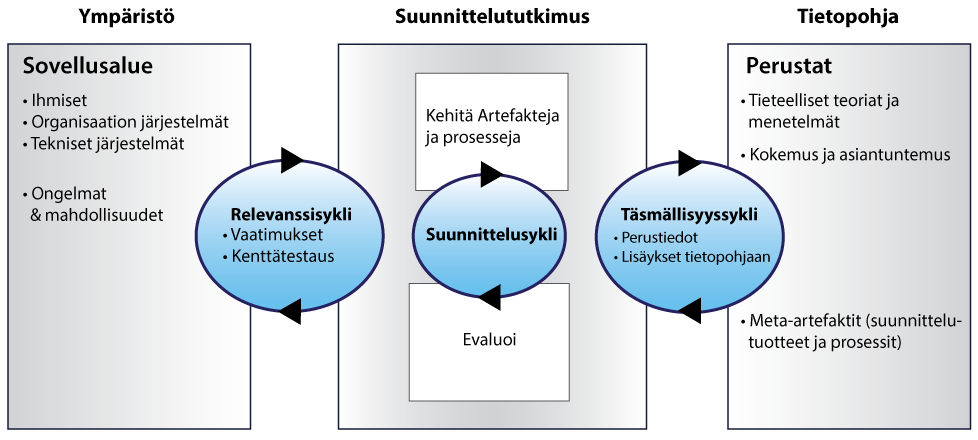
\includegraphics[height=7cm,keepaspectratio]{DSR}
  \caption[]{Suunnittelututkimuksen syklit}
  \label{fig:dsr}
\end{figure}

\subsection{Relevanssisykli}

Relevanssisykli on suunnittelututkimuksen aloittava sykli, joka määrittää sovellusalueen kontekstin tutkimukselle. Sovellusalue koostuu ihmisistä, organisaatiojärjestelmistä ja teknisistä järjestelmistä, jotka toimivat yhdessä tietyn tavoitteen saavuttamiseksi. Suunnittelututkimuksessa on oleellista löytää sovellusalueelta ongelmia tai mahdollisuuksia, joiden pohjalta lähdetään kehittämään niihin erilaisia ratkaisuja artefaktien avulla. Relevanssisykli määrittää ympäristön kautta suunnittelututkimukselle vaatimukset sekä hyväksymiskriteerit tutkimustulosten evaluoinnille. Oleelliset kysymykset ovat: helpottaako artefakti ympäristöään jollain tavalla, ja kuinka tämä parannus voidaan mitata \parencite[][]{cycles}?

Relevanssin toinen merkittävä osa on artefaktin kenttätestaus, joka voidaan suorittaa monin eri tavoin. Sen tarkoituksena on selvittää, täyttääkö artefakti sille määrätyt vaatimukset, ja tuoko se sitä kautta jonkin asteisia parannuksia ympäristöönsä. On myös mahdollista, että vaatimukset ovat alusta alkaen olleet väärät, jolloin ne täytyy uudelleenmäärittää. Suunnittelutukimuksen edetessä tulokset määrittävät sen, vaatiiko tutkimus ylimääräisiä relevanssisyklejä \parencite[][]{cycles}.

Tämän tutkimuksen sovellusalue koostuu yliopistosta organisaationa, opettajista sekä järjestelmistä, joita hyödynnetään äänipalautteen antamisessa. Ensimmäisen relevanssisyklin tärkein tavoite on selvittää, miten opettajat suhtautuvat äänipalautteen antamiseen, millaisia työkaluja he käyttävät sekä millä keinoin äänipalautteen antamista voidaan helpottaa. Relevanssisyklin erityisen tärkeä osa on äänipalautteen antamiseen liittyvien ongelmien tai mahdollisuuksien löytäminen, jotka tämän tutkimuksen kohdalla saivat alkuunsa Heimburgerin, Isomöttösen ym. \parencite[][]{academics} toteuttaman tutkimuksen kautta. Tutkimuksessa opettajat kohtasivat tiettyjä äänipalautteen antamiseen liittyviä ongelmia, jotka herättivät ideoita äänipalautteen antamiseen tarkoitetusta työkalusta.

Kenttätestaus suoritetaan tutkimuksessa kehitettävän prototyyppisovelluksen käyttäjätestaamisella ja evaluoinnilla. Evaluoinnin suorittavat neljä opettajaa, joilla on jo aiempaa kokemusta äänipalautteen antamisesta. Kenttätestauksen suoritukseen osallistuvat tämän tutkielman ohjaajat Anneli Heimburger ja Ville Isomöttönen sekä kaksi muuta yliopistossa työskentelevää opettajaa Paavo Nieminen sekä Harri Keto. Evaluointia käsitellään tarkemmin luvussa X. 

\subsection{täsmällisyyssykli}

Täsmällisyyssyklin tarkoituksena on tuoda tutkimukseen aiempaa tietämystä aihealueeseen liittyen, jotta voidaan varmistua siitä, että toteutettavan suunnittelututkimuksen tulokset ovat innovaatiivisia. Suunnittelututkimus perustuu useimmiten tieteellisiin teorioihin, teknisiin menetelmiin sekä kokemuksiin ja asiantuntijuuteen, jotka määrittävät sovellusalueen sen hetkisen tilan. Lisäksi tietopohjaan kuuluuvat sovellusalueella jo käytössä olevat artefaktit ja prosessit \parencite[][]{cycles}.

Sopivien teorioiden ja menetelmien löytäminen artefaktin kehittämisen ja evaluoinnin tueksi on suunnittelututkimuksen toteuttajien yksi perustavanlaatuisista tehtävistä. On kuitenkin epärealistista ja alalle haitallista odottaa, että kaikki suunnittelututkimuksen osa-alueet perustuvat tiettyihin teorioihin. Suotuisampaa on tunnistaa useita idoiden lähteitä, jotka luovat pohjan suunnittelututkimuksen toteuttamiselle \parencite[][]{cycles}.

Jos suunnittelutukimuksen tulokset ovat innovatiivisia, ne tuovat eri asteisia lisäyksiä sovellusalueen tietopohjaan. Muutoksen voivat liittyä teorioihin, menetelmiin, meta-artefakteihin tai kokemuksiin, jotka on saavutettu tutkimuksen ja kenttätestauksen toteuttamisen yhteydessä \parencite[][]{cycles}.

Tämän suunnittelututkimuksen tietopohja pohjautuu opettajien kokemuksiin ja näkemyksiin äänipalautteen antamisesta, käyttöliittymäsuunnittelussa hyödynnettäviin käytettävyysperiaatteisiin sekä erilaisten audio- ja äänipalauteohjelmistojen tämänhetkiseen tilaan.  Kuten jo aiemmin on mainittu, niin tämä suunnittelututkimus sai alkunsa tutkimuksesta, joka käsittelee äänipalautteen antamista opettajien näkökulmasta. Tutkimuksessa tuli esille tietynlaisia haasteita äänipalautteen antamiseen liittyen, sekä ideoita äänipalautteen antamiseen suunnatusta työkalusta. Jo olemassa olevien nauhoitus- ja äänipalautetyökalujen tutkimisen pohjalta voidaan todeta, että työkalut eivät ole täysin soveltuvia äänipalautteen antamiseen ja sitä kautta niissä on parantamisen varaa. Esimerkiksi useimmat äänipalautteen antamiseen suunnatut työkalut ovat kaupallisia, joten niiden käyttö opetuksessa on lähes aina poissuljettua. Jo tämän tutkimuksen alkuvaiheilla oli selkeää, että äänitteen väliin tulisi pystyä nauhoittamaan uusi äänite mahdollisimman helposti. Monissa äänitystyökaluissa tämä onnistuu, mutta se vaatii useita peräkkäisiä toimintoja. Lisäksi työkalut sisältävät runsaasti sellaisia toimintoja, jotka ovat äänipalautteen antamisessa tarpeettomia. Pelkästään näiden tietojen pohjalta saadaan varmuus siihen, että suunnittelututkimuksessa kehitetään jotain uutta ja innovatiivista.

Käyttöliittymän suunnittelu on erittäin tärkeää, jotta työkalu olisi käytettävyydeltään mahdollisimman hyvä. Suunnittelun apuna tutkimuksessa käytetään kahta toisistaan eroavaa käytettävyysperiaatteiden joukkoa. Nielsenin heuristiikat tarjoavat yleisiä käytettävyyteen liittyviä ohjenuoria kun taas Gestaltin hahmolait keskittyvät käyttöliittymän visuaalisuuteen ihmisaivojen hahmottelukyvyn kautta. Suunnittelussa hyödynnettyjä käytettävyysperiaatteita käsitellään tarkemmin luvussa X.

Äänipalautetyökalun evaluointi suoritetaan hyvin vapaamuotoisena käyttäjäkyselynä, joka suoritetaan kahteen kertaan tutkimuksen eri vaiheissa. Kyselyn tärkein tavoite on saada selville helpottiko äänipalautetyökalu äänipalautteen antamista tai siihen suhtautumista. Lisäksi evaluointiin kuuluu työkalun tarkoituksenmukaisuuden, perustoimintojen sekä käytettävyyden arviointi. Evaluointi on täysin laadullinen, sillä edellä mainittujen ominaisuuksien arvioiminen olisi määrällisesti haastavaa, erityisesti kun kyseessä on keskeneräinen prototyyppisovellus. Äänipalautetyökalun evaluointia käsitellään tarkemmin luvussa X.

\subsection{Suunnittelusykli}

Suunnittelututkimuksen tärkein sykli on suunnittelusykli, joka koostuu artefaktin suunnittelusta ja evaluoinnista. Tarkoituksena on luoda erilaisia suunnittelutyön tuotoksia, arvioida niitä, ja tarkistaa vastaavatko ne relevanssisyklissä määritettyjä vaatimuksia. Artefaktien suunnittelu ja evaluointi toteutetaan täsmällisyyssyklissä määritettyjä teorioita ja mentelmiä hyödyntäen. Suunnittelusyklissä tapahtuu suurin osa suunnittelututkimuksen työstä, ja tästä syystä iteraatioita on tiheämmin kuin relevanssisyklissä tai täsmällisyyssyklissä, jotka luovat pohjan suunnittelusyklissä toteutettaville toimenpiteille \parencite[][]{cycles}.

Suunnuittelusyklissä on tärkeää jakaa vaivannäkö tasaisesti sekä artefaktin kehittämiselle että evaluoinnille, sekä molempien toimintojen tulisi perustua relevanssisyklistä ja täsmällisyyssyklissä määritettyihin teorioihin tai menetelmiin. Suunnittelusykliä joudutaan lähes aina iteroimaan useita kertoja, ennen kuin sen tuloksia voidaan hyödyntää relevanssi ja täsmällisyyssyklissä \parencite[][]{cycles}.

Tässä tutkimuksessa suunnittelusyklien määrä joudutaan rajaamaan kahteen iteraatioon, jotta tutkimuksen laajuus vastaisi tyypillistä pro gradu -tutkielmaa. Ensimmäisen iteraation tavoitteena on kehittää prototyyppi sellaiseen pisteeseen, että äänipalautteen äänittäminen ja editointi olisi mahdollista. Tämä siis tarkoittaa sitä, että työkalun käyttöliittymä, perustoiminnot ja äänileikenäkymä on toteutettu ja testattu tiettyyn pisteeseen. Evaluoinnin tärkein tavoite on löytää äänipalautetyökalun hyvät ja huonot suunnitteluratkaisut, sekä selvittää kaipaako työkalu vielä ylimääräisiä toiminnallisuuksia. Ensimmäisen iteraation suorittavat Anneli Heimburger ja Ville Isomöttönen, jotka toimivat tämän tutkielman ohjaajina. Kaksi muuta koehenkilöä osallistuvat ohjaajien lisäksi vasta toiseen iteraatioon, jossa artefaktiin on tehty muutoksia ensimmäisen iteraation pohjalta.

Näiden kahden suunnittelusyklin lisäksi äänipalautetyökalun kehittäminen tapahtuu useissa pienemmissä sykleissä, jotka muistuttavat varsinaista suunnittelusykliä. Artefaktin suunnitteluratkaisuista neuvotellaan palavereissa ohjaajien kanssa, joilla on kokemusta äänipalautteen antamisesta. Kun suunnitellut ominaisuudet on toteutettu, arvioidaan onko työkalun suunta oikea, ja sovitaan jatkotoimenpiteistä seuraavaa palaveria varten. Tällä syklillä on yhtäläisyyksiä myös relevanssisyklin kanssa, jossa mm. määritellään artefaktin vaatimuksia.

\section{Artefaktin evaluointi}

\subsection{evaluoinnin kriteerit}
\label{kriteerit}

Artefaktin evaluointi on suunnittelututkimuksen merkittävä osa, jossa arvioidaan tietyin menetelmin, täyttääkö artefakti sille määrätyt kriteerit. Suunnittelututkimuksen alkuvaiheilla on tärkeä määrittää mihin objektiin evaluointi kohdistuu ja mitkä ovat evaluoinnin kriteerit, sekä määrittää kuinka artefakti evaluoidaan ja mitä menetelmiä siinä hyödynnetään \parencite[][]{evaluation}. 

Simonin \parencite[][]{simon1996} mukaan suunnitteluartefaktit voidaan mieltää järjestelmiksi. Myös muualla suunnittelututkimukseen liittyvässä kirjallisuudessa artefakteista puhutaan järjestelminä, joten evaluointikriteerien määrittelyssä voidaan hyödyntää systeemiteoriaa \parencite[][]{evaluation}. Systeemiteorian mukaan järjestelmä on suhteessa toisiinsa olevien osien summa, joka luo uusia ominaisuuksia, ja jolla on jokinlainen tavoite \parencite[][]{skyttner}. Järjestelmän kanonisen muodon mukaan järjestelmällä on viisi ulottuvuutta: tavoite, ympäristö, rakenne, aktiivisuus ja evoluutio \parencite[][]{modeling, systemic}.

Edellä mainittuja järjestelmän ulottuvuuksia voidaan hyödyntää artefaktin evaluointikriteerien määrittämisessä.  Prat, Comyn-Wattiau ja Akoka \parencite[][]{evaluation} ovat laatineet evaluaointikriteerien hierarkian, johon on kerätty kirjallisuudessa esiintyviä evaluointikriteerejä. Löydetyt kriteerit on jaoteltu järjestelmän ulottuvuuksien mukaan omiksi ryhmikseen ja osa evaluointikriteereistä on jaettu vielä useampiin alakriteereihin. Evaluointikriteerien hierarkia on esitetty kuviossa ~\ref{fig:evaluointikriteerit}.

\begin{figure}[h]\centering
  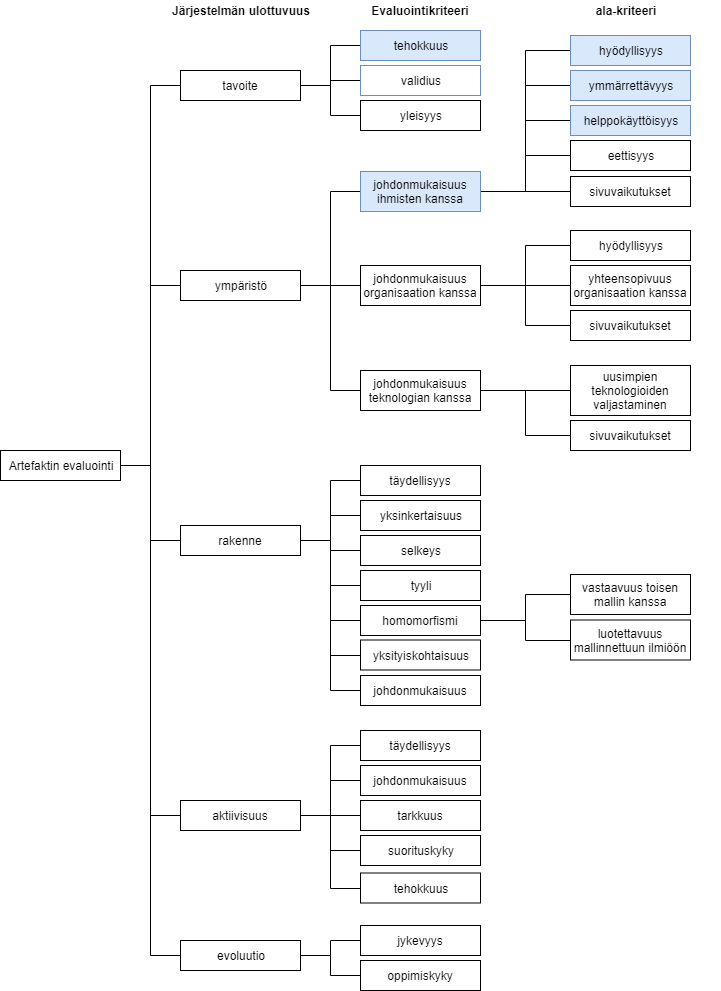
\includegraphics[width=\textwidth,height=\textheight,keepaspectratio]{evaluointikriteerit}
  \caption[]{Evaluointikriteerien hierarkia Pratin, Comyn-Wattiaun ja Akokan \parencite[][]{evaluation} laatimaa kuviota mukaillen. Äänipalautetyökalun evaluoinnin kannalta tärkeimmät evaluointikriteerit on korostettu sinisellä värillä.}
  \label{fig:evaluointikriteerit}
\end{figure}

Järjestelmän ulottuvuuksista tavoitteen alle on luokiteltu seuraavat evaluointikriteerit:  tehokkuus, pätevyys sekä yleisyys. Tehokkuudella mitataan sitä, kuinka hyvin artefakti onnistuu sille määrätyn tavoitteen saavuttamisessa, kun taas pätevyydellä mitataan, toimiiko artefakti oikealla tavalla. Yleisyydellä tarkoitetaan artefaktin tavoitteen laajutta \parencite[][]{evaluation}.

Artefaktin ympäristö koostuu ihmisistä, organisaatioista ja teknologiasta \parencite[][]{hevner2004}. Evaluointikriteereiksi on tästä johtuen määritelty kunkin edellä mainitun osan johdonmukaisuus, jolla tarkoitetaan kunkin osan, tai niistä muodostuvan kokonaisuuden yhteensopivuutta. Nämä evaluointikriteerit on vielä jaoteltu useampiin alakriteereihin, joista sekä ihmisten ja organisaation johdonmukaisuuden alle kuuluva hyödyllisyys mittaa, kuinka laadukkaasti artefakti toimii käytännössä. Ihmisten johdonmukaisuuteen liittyvät muut alakriteerit ovat ymmärrettävyys, helppokäyttöisyys, eettisyys sekä sivuvaikutukset. Organisaation muut johdonmukaisuuden alakriteerit ovat artefaktin yhteensopivuus organisaation kanssa ja sen sivuvaikutukset. Teknologian johdonmukaisuuden alakriteerit ovat uusimpien teknologien valjastaminen ja sivuvaikutukset \parencite[][]{evaluation}.

Järjestelmän rakenteeseen liittyvät evaluointikriteerit ovat artefaktin täydellisyys, yksinkertaisuus, selkeys, tyyli, homomorfismi, yksityiskohtaisuus sekä johdonmukaisuus \parencite[][]{evaluation}. Tämä järjestelmän ulottuvuus liittyy artefakteista malleihin, menetelmiin ja rakennelmiin, joten kriteerejä ei käsitellä sen tarkemmin.

Järjestelmän ulottuvuuksista aktiivisuus liittyy artefaktin toimintaan, ja se sisältää seuraavat evaluointikriteerit: täydellisyys,  johdonmukaisuus, tarkkuus, suorituskyky sekä tehokkuus. Artefaktin toiminnan täydellisyys ja johdonmukaisuus liittyy sekä toiminnalliseen että rakenteelliseen näkökulmaan, ja toiminnan tarkkuus varmistaa sen, että artefaktin tulokset eivät ole ristiriidassa jo olemassa olevien kokeiden kanssa. Suorituskyvyllä tarkoitetaan toiminnan nopeutta tai suoritustehoa, ja tehokkuus mittaa toiminnan syötteiden ja ulostulon välistä suhdetta \parencite[][]{evaluation}.

Järjestelmän evoluutio pitää sisällään evaluaatiokriteereistä jykevyyden (engl. robustness) sekä oppimiskyvyn. Vakaudella tarkoitetaan artefaktin kykyä sopeutua ympäristön muutoksiin ja oppimiskyvyllä sen kykyä oppia asioita aiemmista kokemuksista sekä ympäristön reaktioista \parencite[][]{evaluation}.

Äänipalautetyökalun evaluoinnissa selkeästi tärkeimmät järjestelmän ulottuvuudet ovat tavoite ja ympäristö. Tavoite-ulottuvuuteen sisältyvistä evaluontikriteereistä huomioon otetaan tehokkuus, jolla mitataan sitä, kuinka tehokkaasti artefaktilla pystytään suorittamaan sille oleellinen tehtävä, sekä validius, joka koskee sitä, kuinka oikein artefakti toimii tämän tavoitteen saavuttamisessa. Tehokkuus on kriteereistä tärkein, sillä tutkimuksen tavoitteena on nimenomaan tutkia, voidaanko äänipalautteen antamista helpottaa siihen suunnitellun työkalun avulla. Validiutta tutkimalla tavoitteen saavuttamista voidaan mahdollisesti tehostaa entisestään, joten se on myös oleellinen evaluoinnin kriteereistä. Yleisyys on rajattu evaluointikriteereistä ulkopuolelle, sillä työkalun tavoite on selkeä ja rajattu.

Ympäristö-ulottuvuuden alle kuuluvista evaluointikriteereistä tutkimukseen otetaan johdonmukaisuus ihmisten kanssa, joka on myös yksi evaluoinnin tärkeimmistä kriteereistä. Se jakautuu useampaan alakriteeriin, joista evaluointiin otetaan mukaan hyödyllisyys, ymmärrettävyys ja helppokäyttöisyys. Nämä ovat tärkeitä artefaktin laatuattribuutteja, sillä ne liittyvät suurelta osin käyttäjäkokemukseen, joka taas vaikuttaa käyttäjän suhtautumiseen ja oppimiskynnykseen työkalua koskien. Johdonmukaisuus ihmisten kanssa -evaluointikriteeristä on rajattu ulos eettisyys ja sivuvaikutukset, joilla ei tässä tutkimuksessa ole merkitystä.

Suurin osa suunnittelututkimuksista keskittyy organisaation toiminnan tehostamiseen, mutta tämä tutkimus keskittyy poikkeuksellisesti enemmän ihmisten suhtautumiseen ja kokemuksiin artefaktiin liittyen. Sen lisäksi, koska evaluoitava artefakti on prototyyppi, niin evaluointikriteeri johdonmukaisuus organisaation kanssa rajataan evaluoinnin ulkopuolelle, mutta siihen liittyviä seikkoja voidaan mahdollisesti arvioida evaluoinnin tulosten perusteella välillisesti. 

Rakenteeseen, aktiivisuuteen ja evoluutioon liittyvät evaluointikriteerit voidaan rajata suoraan evaluoinnin ulkopuolelle, sillä evaluoinnin kohteena oleva artefakti on prototyyppi. Ne ovat yksityiskohtaisempia kriteerejä, jotka liittyvät vahvasti mm. viimeistelyyn, täydellisyyteen, suoritustehoon ja mukautuvuuteen, jota ei prototyypiltä voida vaatia. Äänipalautteen suunnittelussa ja toteutuksessa nämä seikat on myös jätetty lähes täysin huomiotta, sillä tarkoituksena on kahden tutkimusiteraation kautta saada selville työkalun toimivat ja ei-toimivat ratkaisut tavoitteeseen ja käyttäjäystävällisyyteen liittyen.

\subsection{Artefaktin evaluointimenetelmät}

Artefaktin evaluointi voidaan suorittaa useilla eri menetelmillä.  Prat, Comyn-Wattiau ja Akoka \parencite[][]{evaluation} ovat omassa suunnittelututkimuksessaan luoneet mallin, joka kuvaa evaluointimenetelmän erilaisia ominaisuuksia. He ovat jaotelleet evaluointimenetelmän kokonaisuudessaan viiteen eri komponenttiin, joita ovat evaluointikriteerit, evaluoinnin tyyppi, evaluoinnin taso, evaluoinnin suhteellisuus sekä toissijaiset osallistujat. Evaluoinnin kriteerit on käsitelty edellisessä alaluvussa \ref{kriteerit}. Evaluoinnin tyyppi jaotellaan joko määrälliseksi tai laadulliseksi, joista määrällinen tuottaa jonkin mitatun tai havaitun numeerisen arvon \parencite[][]{evaluation}. Evaluointi voi olla joko abstrakti- tai instanssi-tasoinen, joka riipuu evaluoitavan artefaktin ominaisuuksista. Instanssitasoinen evaluointi voidaan suorittaa, joko kuvitteellisten tai autenttisten tehtävänantojen kautta. Evaluointi voi olla suhteellisuudeltaan absoluuttinen, suhteessa samankaltaisiin artefakteihin tai suhteessa artefaktin puuttumiseen. Toissijaiset osallistujat taas ovat henkilöitä, jotka testaavat esimerkiksi artefaktin prototyyppiä \parencite[][]{evaluation}. Edellä mainituista evaluoinnin ominaisuuksista osa jakautuu vielä alaluokkiin.

Tässä tutkimuksessa suoritettava äänipalautetyökalun evaluointi on instanssitasoista, sillä abstraktin artefaktin sijaan evaluoinnin kohteena on prototyyppi äänipalautetyökalusta. Usein prototyyppiä evaluoidessa hyödynnetään toissijaisia osallistujia, mutta tämän tutkimuksen tapauksessa artefaktia evaluoivat ainoastaan ensisijaiset koehenkilöt. Ensimmäiseen iteraatioon osallistuu kaksi henkilöä, ja toiseen iteraatioon neljä henkilöä.

Molemmat evaluointikerroista suoritetaan lähes samalla tavalla, pieniä muutoksia lukuunottamatta. Koehenkilöille lähetetään sähköpostin välityksellä linkki äänipalautetyökaluun, sekä arviointilomakkeeseen, jossa heidän tulee vastata äänipalautetyökalua koskeviin kysymyksiin. Evaluoinnin ohjeistukset on kerrottu arviointilomakkeen alussa. Koehenkilöitä pyydetään aluksi käyttämään äänipalautetyökalua autenttisessa tilanteessa, jotta evaluoinnin tulokset olisivat mahdollisimman tarkkoja. Koehenkilöt voivat suorittaa testauksen, joko mobiililaitteella, tabletilla tai tietokoneella, sillä työkalun tarkoituksen on toimia joustavasti alustasta tai laitteesta riippumatta. Koekäytön jälkeen heitä pyydetään testaamaan jokaista työkalun perustoimintoja, joita annetun tehtävän aikana koehenkilö ei testannut. Nämä kaksi tehtävänantoa suoritettuaan koehenkilön tulee vastata lomakkeella esitettyihin kysymyksiin. 

Lomakkeella käyttäjän tulee arvioida, palveliko äänipalautetyökalu tarkoitustaan, helpottiko työkalu äänipalautteen antamista entuudestaan, tai muuttiko se suhtautumista äänipalautteen antamiseen. Sen lisäksi koehenkilön tulee arvioida työkalun perustoiminnallisuuksia, jos joitakin huomioita niihin liittyen ilmaantuu. Lomakkeen viimeisissä osioissa käyttäjällä on mahdollisuus tuoda vapaamuotoisesti ilmi työkaluun liittyviä huomioita ja kehitysideoita.

Evaluointi on suhteeltaan absoluuttinen, suhteessa muihin samankaltaisiin artefakteihin, sekä suhteessa vastaavanlaisten artefaktien puuttumiseen, joten se kattaa kaikki kolme osa-aluetta. Evaluoinnissa arvioidaan absoluuttisesti työkalun tarkoituksenmukaisuutta ja toiminnallisuutta, mutta lisäksi äänipalautteen antoa pyydetään vertaamaan koehenkilön aiempiin kokemuksiin. Toisaalta aivan vastaavanlaisia äänipalautteen antamiseen suunniteltuja artefakteja ei ole vielä kehitetty, joten vertaaminen tapahtuu esimerkiksi perinteisiä nauhoitusohjelmia vasten.

\begin{table}[t]
\caption{Yhteenveto evaluoinnista}
\begin{tabular}{|l|l|l|l|l|}
\hline
Kuvaus                                                                                                                                         & evaluointikriteerit                                                                                                                                                                             & \begin{tabular}[t]{@{}l@{}}evaluoinnin\\  tyyppi\end{tabular} & \begin{tabular}[t]{@{}l@{}}evaluoinnin\\ taso\end{tabular} & \begin{tabular}[t]{@{}l@{}}evaluoinnin \\ suhteellisuus\end{tabular}                                                                                  \\ \hline
\begin{tabular}[t]{@{}l@{}}Äänipalautetyökalun\\ tarkoituksenmukaisuuden, \\ käytettävyyden ja \\ toiminnallisuuden\\ evaluointi.\end{tabular} & \begin{tabular}[t]{@{}l@{}}Tavoite / tehokkuus\\ Tavoite / validius\\ \\ ympäristö / \\ johdonmukaisuus\\ ihmisten kanssa /\\ hyödyllisyys,\\ ymmärrettävyys, \\ helppokäyttöisyys\end{tabular} & Laadullinen                                                   & Instanssi                                                  & \begin{tabular}[t]{@{}l@{}}Absoluuttinen,\\ \\ suhteessa saman-\\ kaltaisiin\\ artefakteihin,\\ \\ suhteessa artefaktien \\ puuttumiseen\end{tabular} \\ \hline
\end{tabular}
\end{table}

\chapter{Työkalun suunnittelu ja toteutus}

Tässä luvussa käsitellään äänipalautetyökalu-prototyypin suunnittelua ja toteutusta eri näkökulmista. Aluksi läpikäydään työkalun tekniseen toteutukseen liittyviä seikkoja, jonka jälkeen käsitellään käyttöliittymän suunnitelua ohjaavia käytettävyyysperiaatteita sekä itse käyttöliittymää. Lopuksi esitetään työkalun perus- ja erikoistoiminnot, ja kuinka näihin toiminnallisuuksiin päädyttiin.

Työkalu suunniteltiin pääasiassa yhteistyössä pro gradu -ohjaajien kanssa, joilla molemmilla on kokemusta äänipalautteen antamisesta. He ovat myös olleet osallisina tutkimuksessa, jossa selvitettiin akateemikkojen suhtautumista äänipalautteen antamiseen. Tutkimuksessa kolmella neljästä koehenkilöstä heräsi ideoita työkalusta, jolla äänipalautetta voisi antaa, editoida, hallita ja arkistoida \parencite[][]{academics}. Edellä mainitun tutkimuksen, sekä ohjaajien omien kokemusten ja näkemysten pohjalta äänipalautetyökalun suunnittelu ja toteutus päätettiin aloittaa.

\section{Tekniset toteutusratkaisut}

Äänipalautetyökalun yksi tärkeimmistä vaatimuksista oli se, että sitä voidaan käyttää vaivattomasti laitteella kuin laitteella ilman erillistä asennusta. Tämän vuoksi työkalu toteutettiin web-pohjaisena sovelluksena, eli sitä pystytään käyttämään selaimen välityksellä tietyn www-osoitteen kautta. Jotta tämä onnistuisi, sovelluksen täytyy sijaita jollain palvelimella. Ensimmäisen iteraation ajan työkalu oli sijoitettuna Google App Engine -palveluun, mutta kokeilujakson päätyttyä se siirrettiin Heroku-palveluun, joka tarjoaa web-sovellusten verkkoisännöintiä täysin maksutta. 

Työkalu toteutettiin yhdestä näkymästä koostuvana staattisena verkkosivuna, sillä siten protoyyppi saadaan valmiiksi kaikista nopeiten. Web-pohjaisuuden takia sovelluksen toteutustekniikat olivat selkeitä: rakenteen toteutuksessa käytetään HTML-merkintäkieltä, elementtien asettelussa CSS3-tyyliohjeita sekä toiminnallisuuksien toteutuksessa JavaScript-ohjelmointikieltä. Javascript-kehityksessä hyödynnetään jQuery-kirjastoa helpottamaan tiettyjä toimenpiteitä, kuten DOM-elementtien manipulointia. JQueryn lisäksi kehityksessä ei hyödynnetty muita kirjastoja tai ohjelmistokehyksiä, sillä ylimääräisistä riippuvuuksilta haluttiin välttyä jatkokehitystä ajatellen. Ääniaallon piirtämiseen harkittiin wavesurfer-kirjastoa, mutta sen integrointi äänipalautetyökaluun olisi vaatinut enemmän aikaa, kuin sen toteuttaminen itse verkosta haettujen ohjeiden avulla.

Työkalun nauhoitus on toteutettu Mediarecorder API-ohjelmointirajapintaa hyödyntäen, joka mahdollistaa äänen ja videon kaappaamisen tietovirtana selaimen kautta. Tutkimuksen toteutushetkellä selainten tuki kyseiselle ohjelmointirajapinnalle ei ole täysin kattava, sillä Safari-selaimen eri versiot tukevat sitä ainoastaan osittain. Nauhoittaminen oltaisiin voitu tehdä myös vaihtoehtoisella tavalla, joka olisi mahdollistanut nauhoittamisen useammilla selaimilla, mutta se rajattiin toteutuksen ulkopuolelle, sillä tärkeintä on, että prototyyppiä päästään testaamaan ainakin tietyillä eniten käytetyimmillä selaimilla.

\section{Hyödynnetyt käytettävyysperiaatteet}

Äänipalautetyökalun suunnittelussa ja käytettävyyden arvioinnissa on hyödynnetty erilaisia heuristiikkoja, jotta käytettävyys saataisiin mahdollisimman korkealle tasolle. Hyödynnetyt käytettävyysperiaatteet ovat Gestaltin hahmolait, jotka käsittelevät erilaisten kuvioiden ja kokonaisuuksien visuaalisten hahmottamista sekä käytettävyysguru Jakob Nielsenin laatimat käytettävyysheuristiikat, jotka ovat vakiinnuttaneet asemansa käytettävyyden saralla jo 90-luvulta saakka.

Käytettävyydellä on suuri merkitys ohjelmistojen suunnittelussa ja arvioinnissa. Käytettävyydellä tarkoitetaan laatuattribuuttia, jolla mittataan sitä, kuinka helppokäyttöinen käyttöliittymä on. Sillä myös viitataan kehitysprosessin aikaisiin toimiin, joilla pyritään parantamaan käyttöliittymän helppokäyttöisyyttä \parencite[][]{intro-usability}.

Nielsenin \parencite[][]{intro-usability} mukaan käytettävyys voidaan määrittää viidellä eri laatukomponentilla: opittavuudella, tehokkuudella, muistettavuudella, virheiden tekemisellä ja niistä toipumisella sekä käyttömukavuudella. Opittavuudella tarkoitetaan sitä, kuinka helppo käyttäjän on ensimmäistä kertaa käyttöliittymän kohdattaessaan suorittaa erilaisia perustoimenpiteitä ja tehokkuudella sitä, kuinka nopeasti nämä toimenpiteet suoritetaan. Muistettavuudella tarkoitetaan sitä, kuinka nopeasti käyttäjä pystyy uudelleensaavuttamaan käyttötehokkuuden tietyn pituisen tauon jälkeen. Virheiden tekeminen ja niistä toipuminen kattaa käyttäjän tekemien virheiden kokonaismäärän, kuinka vakavia ne ovat sekä kuinka helposti näistä virheistä voidaan toipua. Käyttömukavuudella tarkoitetaan sitä, kuinka miellyttväksi käyttöiittymän käyttäminen koetaan.

Edellämainittujen laatuattribuuttien lisäksi on myös monia muita tärkeitä laatuattribuutteja, joista yksi on hyödyllisyys. Sillä mitataan, kuinka hyvin käyttöliittymän avulla pystytään tekemään juuri se, mitä käyttäjä tarvitsee \parencite[][]{intro-usability}. Se onkin tässä tutkimuksessa toteutetun äänipalautetyökalun käytettävyyden arvioinnissa erittäin tärkeässä roolissa, sillä työkalun käyttötarkoitus on hyvin tarkkarajainen. Tässä tutkielmassa hyödyllisyydestä puhutaan tarkoituksenmukaisuutena, sillä se on suomennettuna kuvaavampi termi.


\subsection{Gestaltin hahmolait}

Gestaltin hahmolait ovat periaatteita, jotka selittävät, kuinka ihmisaivot ryhmittelevät yksittäiset visuaaliset elementit näkemästään ympäristöstä \parencite[][]{koffka}. Hahmolait perustuvat 1800-luvulla alkunsa saaneeseen Gestalt-psykologiaan, joka tutkii kokonaisuuden ymmärtämistä sen yksittäisten osiensa sijaan. Max Wertheimerin vuonna 1923 julkaisemassaan artikkelissa "Untersuchungen zur Lehre von der Gestalt. II", hän käsittele havaisemiseen liittyviä lakeja ja niiden perusongelmia. Sillä oli merkittävä vaikutus Gestalt-psykologiaan ja myös muihin tieteenaloihin, joten sitä voidaan pitää hahmolakeihin liittyvän kirjallisuuden yhtenä merkittävimpänä julkaisuna \parencite[][]{rearranged}. 

Ajan saatossa Gestaltin hahmolaeista on ilmestynyt lukuisia eri variaatioita, mutta ne ovat usein keskenään samankaltaisia ja sisältävät päällekäisyyksiä. Koska Gestalt-psykologiaa voidaan soveltaa useisiin eri tarkoituksiin, niin hahmolaeista joudutaan usein valitsemaan sopivimmat vaihtoehdot tapauskohtaisesti. Chang ym. \parencite[][]{chang}, ovat koonneet tutkimukseeensa 11 hahmolakia, jotka ovat oletetusti hyödyllisimpiä opetuskäyttöön tarkoitetun ohjelmiston visualisessa suunnittelussa. Nämä hahmolait ovat kaikenkaikkiaan:

\begin{enumerate}
  \item Symmetrian laki
  \item Jatkuvuuden laki
  \item Sulkeutuvuuden laki
  \item Kohteen ja alustan laki
  \item Keskipisteen laki
  \item Yhdenmukaisuuden laki
  \item Hyvän muodon laki
  \item Läheisyyden laki
  \item Samankaltaisuuden laki
  \item Yksinkertaisuuden laki
  \item Yhtenäisyyden laki
\end{enumerate}

Symmetrian lain mukaan symmetrinen kuvio havainnoidaan kokonaisuudeksi sen osien sijaan sitä vahvemmin, mitä symmetrisempi kuvio on. Jatkuvuuden lain mukaan taas viivat, jotka jatkavat risteyskohdasta mahdollisimman samaan suuntaan, koetaan samaksi viivaksi. Sulkeutuvuuden lain mukaan kuvio tulkitaan kokonaisuudeksi, vaikka siitä puuttuisi osia. Kohteen ja alustan lain mukaan kohde ja sen alusta tulkitaan eri tavalla väreistä riippuen. Keskipisteen lain mukaan jokin muista erottuva kokonaisuus vie käyttäjän huomion, ja ohjaa sitä tiettyyn suuntaan. Yhdenmukaisuuden lain mukaan kuviot tulkitaan aiempien kokemuksien perusteella, eli se vastaa Nielsenin heuristiikoista yhdenmukaisuutta ja standardeja. 

Äänipalautetyökalun käyttöliittymä on yksinäkymäinen staattinen verkkosivu, joka koostuu  äänileikenäkymästä sekä perustoimintojen ja erikoistoimintojen painikkeista. Koska käyttöliittymän on tarkoitus olla mahdollisimman yksinkertainen, kaikkia edellä mainittuja heuristiikkoja tuskin tullaan hyödyntämään käyttöliittymäsuunnittelussa, mutta ne on silti hyvä olla ylöskirjattuna, sillä niitä voidaan hyödyntää äänipalautetyökalun mahdollisessa jatkokehityksessä. 

\subsection{Nielsenin heuristiikat}

Jakob Nielsen on yksi maailman tunnetuimmista käytettävyysasijantuntijoista, joka on työskennellyt käytettävyyyden parissa 90-luvulta saakka. Jakob Nielsen ja Rolf Molich \parencite[][]{improving-human} määrittelivät vuonna 1990 yhdeksän erilaista käytettävyysheuristiikkaa järjestelmän käytettävyyden arviointiin. Nielsen \parencite[][]{enhancing} jalosti näistä vuonna 1994 päivitetyn listauksen, joka on validi ja laajasti käytössä oleva yhä lähes kaksikymmentä vuotta myöhemmin. 

Käyttöliittymien käytettävyyden arviointi toteutetaan useimmiten heuristisesti, eli käyttöliittymää tarkastellaan ja siitä koitetaan löytää toimivat ja ei-toimivat ominaisuudet. Se on halpa ja intuitiivinen tapa löytää käyttöliittymän käytettävyysongelmia, eikä se vaadi erityistä etukäteissuunnittelua. Lisäksi sitä voidaan käyttää jo varhaisessa vaiheessa suunnitteluprosessia ja ihmisten motivointi arvioinnin suorittamiseen on helppoa \parencite[][]{heuristic-evaluation}.

Jotkut suorittavat heuristisen arvioinnin oman intuition tai maalaisjärjen pohjalta, mutta Nielsen ja Molich hyödyntävät siinä itse-laatimiaan heuristiikkojansa, jotka kattavat erittäin suuren osan käytettävyyteen liittyvistä ongelmista \parencite[][]{heuristic-evaluation}. Nielsenin heruristiikkojen lisäksi on olemassa useita muita käytettävyysheuristiikkoja, joten parhaiden käytettävyysheuristiikkojen määrittäminen on avoin kysymys \parencite[][]{enhancing}. 

Heuristisessa evaluoinnissa ei tulisi luottaa ainoastaan yhden ihmisen arviointiin, vaan arvioijia olisi hyvä olla noin kolmesta viiteen \parencite[][]{heuristic-evaluation}. Tässä tutkimuksessa suoritettava evaluointi ei kuitenkaan perustu heuristiikkoihin, sillä tärkein tavoite on selvittää, kuinka hyvin äänipalautetyökalu suoriutuu nimenomaan äänipalautteen antamisesta, eikä niinkään yleisestä käytettävyydestä. Heuristiikkoja on kuitenkin käytetty apuna työkalun käyttöliittymän toiminnallisuuksien suunnittelussa, mutta ne eivät sisälly varsinaiseen työkalun evaluointiin.


% Table generated by Excel2LaTeX from sheet 'Sheet1'
\begin{table}[htbp]
  \centering
  \caption{Ei meinaa sisältö mahtua. pitäisikö kukin heuristiikoista olla ala-otsikkoina?}
    \begin{tabular}{p{12.355em}p{21.855em}}
    \multicolumn{1}{l}{\textbf{Järjestelmän tilan näkyvyys}} & Järjestelmän tulisi informoida käyttäjälle tapahtumista asianmukaisilla palautteilla riittävän nopeasti. \\
    \textbf{Järjestelmän ja reaalimaailman yhtenäisyys} & Järjestelmän kielellisen sisällön tulisi olla käyttäjän ymmerrättävissä. Tiedon tulisi myös näyttäytyä luonnollisessa ja loogisessa järjestyksessä. \\
    \multicolumn{1}{l}{\textbf{Käyttäjän hallinta ja vapaus}} & Käyttäjät tekevät usein virheitä, joten ei-toivotusta tilasta tulisi päästä pois helposti esim. peruuta- ja palauta -toiminnoilla. \\
    \multicolumn{1}{l}{\textbf{Yhdenmukaisuus ja standardit}} & Erilaisten sanojen, tilanteiden ja toimintojen tulisi olla yhdenmukaisia, ja Järjestelmän tulisi myös noudattaa tunnettuja käytänteitä. \\
    \multicolumn{1}{l}{\textbf{Virheiden estäminen}} & Järjestelmän tulisi ensisijaisesti toimia siten, että virheitä ei pääsisi tapahtumaan. Virheelle alttiissa tilanteessa käyttäjältä tulisi pyytää varmistus toimenpiteen jatkamisesta. \\
    \textbf{Tunnistaminen muistamisen sijaan} & Käyttäjän muistamisen tarve tulisi minimoida pitämällä oleelliset objektit, toiminnot ja valinnat näkyvillä. Ohjeet järjestelmän käyttämiseen tulisi olla myös joko näkyvillä tai helposti saatavilla. \\
    \multicolumn{1}{l}{\textbf{Joustavuus ja käytön tehokkuus}} & Oikopolkut erilaisille toimenpiteille nopeuttaa usein järjestelmän käyttöä, joten niiden tarjoaminen kokeneemmille käyttäjille on usein kannattavaa.  \\
    \textbf{Esteettisyys ja minimalistinen suunnittelu} & Tarpeetonta informaatiota dialogeissa tulisi välttää, sillä se vie näkyvyyttä relevantilta informaatiolta. \\
    \textbf{Virheiden tunnistaminen ja virheistä toipuminen} & Virheviestien tulisi olla selkokielisiä, sekä niiden tulisi täsmällisesti osoittaa millainen virhe on kyseessä ja miten siitä pystytään toipumaan. \\
    \textbf{Avustus ja dokumentaatio} & Dokumentaation tarjoaminen on useimmiten tarpeen, ja käyttäjän tulisi pystyä löytämään sieltä kaikki tarvittava informaatio pystyäkseen käyttämään järjestelmää. \\
    \end{tabular}%
  \label{tab:addlabel}%
\end{table}%

\begin{center}
\begin{tabular}[t]{|p{5cm}|p{5cm}|}
    \hline
    Järjestelmän tilan näkyvyys  & Järjestelmän tulisi informoida käyttäjälle tapahtumista asianmukaisilla palautteilla riittävän nopeasti. \\
    \hline
	Järjestelmän ja reaalimaailman yhtenäisyys  & asdasdasdas asdasd asd asd \\
    \hline
\end{tabular}
\end{center}


\section{Käyttöliittymä}

- Mahd. yksinkertainen käyttöliittymä. Käytettävyys estetiikan edellä, sillä prototyyppi.

Käyttöliittymä on järjestelmän osa, jonka kautta käyttäjä on vuorovaikutuksessa järjestelmän kanssa saavuttaakseen tietyn tavoitteensa \parencite[][]{stone}. Äänipalautetyökalun tapauksessa käyttötarkoitus on hyvin rajattu äänipalautteen antamiseen, joten käyttöliittymän on tuettava juuri sitä mahdollisimman tehokkaasti ja käyttäjäystävällisesti.  Käyttöliittymissä on usein myös eroja erilaisten järjestelmien välillä, sillä vuorovaikutuksessa käytetään erilaista välineitä, jotka vaikuttavat käyttöliittymäsuunnitteluun \parencite[][]{stone}. Äänipalautetyökalun yksi tärkeimmistä vaatimuksista on se, että se on käytettävissä perinteisillä tietokoneilla, tableteilla ja puhelimilla, joten myös käyttöliittymä on suunniteltava siten, että sen käyttö onnistuu hiiren ja näppäimistön lisäksi myös kosketusnäytöllä. Myös käyttöliittymän skaalautuvuus on otettava huomioon, sillä päätelaitteiden ruudun koko vaikuttaa merkittävästi siihen, kuinka käyttöliittymän komponentit järjestestäytyvät. Käyttöliittymä on esitetty tietokone-koossa kuvassa X, tablettikoossa-kuvassa X ja mobiili-koossa kuvassa X.

Käyttöliittymän suunnittelun apuna hyödynnetään usein erilaisia käytettävyysperiaatteita, joilla käyttöliittymän suunnitteluratkaisuja voidaan perustella. Äänipalautetyökalun käyttöliityymän suunnittelussa on hydynnetty Nielsenin heuristiikkoja sekä Gestaltin hahmolakeja, jotka on käsitelty tarkemmin luvussa X. Tässä luvussa esitellään äänipalautetyökalun käyttöliittymä kokonaisuudessaan, ja peilataan tehtyjä suunnittelu- ja toteutusratkaisuja hyödynnettyihin käytettävyysperiaatteisiin. Luvussa ja kuvissa esitettävä käyttöliittymä on suunnittelututkimuksen toisessa iteraatiossa evaluoitu konfiguraatio, joten siinä on pieniä muutoksia ensimmäisen evaluoinnin kohteena olevaan käyttöliittymään verrattuna. 

Äänipalautetyökalun käyttöliittymä voidaan jakaa vaakasuunnassa neljään eri alueeseen, joista kulkin eroaa selvästi toisistaan. Työkalun yläosassa sijaitsevat avustusikkunan avaava kysymysmerkki-ikoni, siniset erikoistoiminto-painikkeet sekä peruuta- ja palaa-toiminnot. Keskiössä sijaitsee muusta taustasta selkeästi erottuva äänileikenäkymä, joka on käytännössä aikajana, johon nauhoitetut äänileikkeet ääniaaltoineen piirretään. Äänileikenäkymän alapuolella sijaitsevat navigaatiotoiminnot, jotka toteutettiin ensimmäisen iteraation evaluointitulosten pohjalta. Alimpana käyttöliittymässä sijaitsevat perustoiminnot, joiden avulla varsinainen äänipalautteen nauhoittaminen ja editointi suoritetaan. 

Edellä mainittujen osioiden sijoittelulla ja ulkoasulla on suuri merkitys työkalun käytettävyyden kannalta, jotta ne erottuisivat selkeästi erilaisiksi kokonaisuuksisi, joilla on oma tehtävänsä. Käyttöliittymän komponenttien asettelu on tehty mahdollisimman symmetriseksi ja tasapainoiseksi kokonaisuudeksi, ilman että yhtäkään toiminnallisuutta olisi piilotettu käyttäjältä. Gestaltin symmetrian lain mukaan tasapainoinen, eli keskiviivan molemmin puoleinen asettelu koetaan selkeämmäksi, kuin epäsymmetrinen asettelu. Nielsenin tunnistaminen muistamisen sijaan -heuristiikan mukaan taas käyttöliittymän toiminnallisuuksien tulisi olla esillä ja mahdollisimman helposti saatavilla, joka myös toteutuu käyttöliittymässä. Edellä mainittujen seikkojen lisäksi käyttöliittymä on suunniteltu visuaalisuudeltaan mahdollisimman selkeäksi, eikä se sisällä epäolennaista informaatiota, joten se on linjassa myös Nielsenin esteettinen ja minimalistinen suunnittelu -heuristiikan kanssa. Informaation määrää on vähennetty myös tietoisesti siten, että perustoiminnot ovat painikkeita, jotka toimivat kuten kytkimet, eli kun toiminto aktivoidaan, muut perustoiminnot muuttuvat haaleiksi merkiksi siitä, että ne eivät sillä hetkellä ole käytettävissä. Lisäksi aktivoidun painikkeen teksti muuttuu tällöin esimerkiksi Play-toiminnon tapauksessa "Stop"-tekstiksi.

Gstaltin läheisyyden lain mukaan vierekkäin olevat elementit tulkitaan yhteenkuuluviksi, jonka vuoksi sitä on hyödynnetty käyttöliittymän painikkeiden ryhmittelyssä. Käyttöliittymän erikoistoiminnot, peruuta - ja palaa-komennot, navigointipainikkeet sekä perustoiminnot ovat toiminnallisuuksiltaan selkeästi toisistaan eroavia, joten ne on ryhmitelty eri tavoin äänileikenäkymän ympärille. Perustoiminto-painikkeet muodostavat oman ryhmänsä, mutta niiden sisäisessä jaottelussa on myös hyödynnetty läheisyyden lakia. Record-, ja Insert Record -toiminnot ovat selvästi nauhoitukseeen liittyviä toimintoja, joten ne on oma pienempi ryhmänsä. Play- ja Previe-toiminnot taas ovat äänitteiden toistamiseen liittyviä toimintoja, joten ne ovat oma ryhmänsä. Split- ja Delete-toiminnot liittyvät äänileikkeiden katkomiseen ja poistamiseen, joten myös ne ovat vahvasti liitoksissa toisiinsa. Läheisyyden lakia hyödyntäen, nämä kolme perustoimintojen ryhmää ovat erotettu toisistaan suuremmilla väleillä, kun toistensa kanssa samankaltaiset perustoiminnot. 

Gestaltin läheisyyden lain lisäksi elemettejä voidaan ryhmitellä myös samanlaisuuden lakia hyödyntäen. Kohteet voidaan tulkita samanlaiseksi, joko värin, koon, muodon perusteella. Äänipalautetyökalussa värin avulla ryhmittelyä on hyödynnetty erityisesti painikkeissa, läheisyyden lain lisäksi. Erikoistoiminnot ovat korostettu sinisellä värillä, kun taas perustoiminnot ja niihin vahvasti niittyvät peruuta- ja palaa -toiminnot on värjätty harmaalla värillä. Navigointipainikkeet taas on väriltään myös äänileikenäkymässä käytetty vaalean harmaa, sillä ne liittyvät vahvasti äänileikenäkymään, jossa äänileikkeiden välillä navigointi tapahtuu. Muista painikkeista eroten navigointipainikkeet on myös suorakaiteen sijasta ympyrän muotoisia, jotta ne erottuisivat selkeästi niiden alapuolella sijaitsevista perustoiminnoista. Koska uloimpien ja sisempien navigointipainikkeiden toiminnallisuuksissa on eroja, niin kaksi sisimmäistä painiketta on kooltaan suurempia, kuin kaksi ulommaista painiketta. Lisäksi ulommissa ja sisemmissä painikkeissa olevien nuolien tyyli on hieman erilainen, jotta ne erottuisivat toisistaan.

Kaikissa käyttöliittymän painikkeissa, erikoistoiminnot poislukien, on hyödynnetty ikoneja, jotta ne olisivat mahdollisimman helposti ymmärrettäviä. Nielsenin johdonmukaisuus ja standardit -heuristiikan sekä Gestaltin yhdenmukaisuuden lain mukaan käyttöliittymässä tulisi käyttää tuttuja kuvioita, joiden tulkintaa helpottavat aiemmat kokemukset. Suurimmassa osassa ikoneista tämä toteutuu ainakin suurimmaksi osaksi, mutta esimerkiksi Insert Record on uudenlainen toiminto, jota ei ole saatavilla äänitystyökaluissa, joten ikoni täytyi kehitellä itse. Johdonmukaisuutta ja standardeja koskeva nielsenin heuristiikka koskee kuvioiden lisäksi myös tekstiä, joten painikkeiden teksteissä on pyritty noudattamaan standardeja. Poikkeuksena ovat Insert Record -, ja preview-toiminnot, joille jouduttiin keksimään nimi itse. Insert Record-toiminnosta joku voi päätellä, että kyseessä on väliin nauhoittaminen, sillä insert-toiminto löytyy myös näppäimistöstä, mutta Preview-toiminto voi olla vaikeampi päätellä pelkän tekstin pohjalta. Nielsenin heuristiikkojen mukaan järjestelmässä tulisi puhua käyttäjän ymmärtämää kieltä, johon painikkeiden teksteillä ja avustusikkunan toimintojen kuvauksilla pyritty.

Johdonmukaisuutta ja standardeja on myös pyritty noudattamaan äänileikenäkymässä, joka koostuu aikajanasta, kursorista, äänileikkeistä ja vierityspalkista. Kuten useimmissa ohjelmistoissa, aikajana on äänileikenäkymän yläreunassa, jonka alla on kaistale, jossa äänileikkeet näytetään. Aikajanaa tai äänileikettä klikattessa punaisella värillä korostettua äänileikenäkymän kursoria siirrteään klikattuun kohtaan. Äänileikkeisiin piirretään äänen visuaalisen hahmottamisen tueksi ääniaalto, kuten useimmissa äänitystyökaluissa on tapana. Yksittäisen äänileikkeen reuna on ohut ja saman värinen kuin piirrettävä ääniaalto, joten äänileikkeiden erottamisen tueksi, äänileikettä klikkaamalla, se korostetaan sinisen tummemmalla sävyllä.

Nielsenin käyttäjän hallinta ja vapaus -heuristiikan mukaankäyttäjän tulisi pystyä palaamaan ei-toivotusta tilasta, joten työkaluun on toteutettu peruuta- ja palaa-toiminnot. Nielsenin heuristiikkojen mukaan käyttöliittymän tulisi olla myös joustava ja tehokas, joten tietyille toiminnoille on määritetty pikanäppäimet. Peruuta- ja palauta-toiminnoissa on noudatettu yleistä "CTRL + Z" ja "CTRL + Y" näppäinyhdistelmää, ja Delete-toiminnossa delete-näppäintä. Perustoiminnoille pikanäppäinten määrittämistä harkittiin, mutta tässä tutkimuksessa ainoastaan Play-toiminto aktivoituu välilyöntiä painamalla. Äänileikenäkymässä on alusta asti ollut mahdollisuus liikuttaa kursoria myös nuolinäppäimillä, mutta ensimmäisen iteraation jälkeen toteutettuihin yksittäisten äänileikkeiden välillä navigointitoimintoihin lisättiin koehenkilön ehdottama "SHITF + NUOLI OIKEALLE TAI VASEMMALLE" näppäinyhdistelmä.

Lisäksi Nielsenin heuristiikkojen mukaan virheiden tapahtuminen tulisi ensisijaisesti estää, ja sellaisen sattuessa, virheestä tulisi esittää selkeä kuvaus ja ohjeet siitä toipumiseen. Koska evaluoitava äänipalautetyökalu on prototyyppi, niin virheitä saattaa käytön aikana kuitenkin ilmaantua. Toisen iteraation evaluoinnin ensimmäisenä suorittanut henkilö huomasi käyttöliittymää vilkaistessaan, ennen ohjeistuksen lukemista, ettei erikoistoiminnoista tapahtunut mitään, ja informoi asiasta. Tämän vuoksi erikoistoimintojen painikkeisiin lisättiin sellainen toiminto, että niitä painettaessa ilmoitetaan käyttäjällä ponnahdusikkunana, että niitä toimintoja ei ole toteutettu.

\begin{figure}[h]\centering
  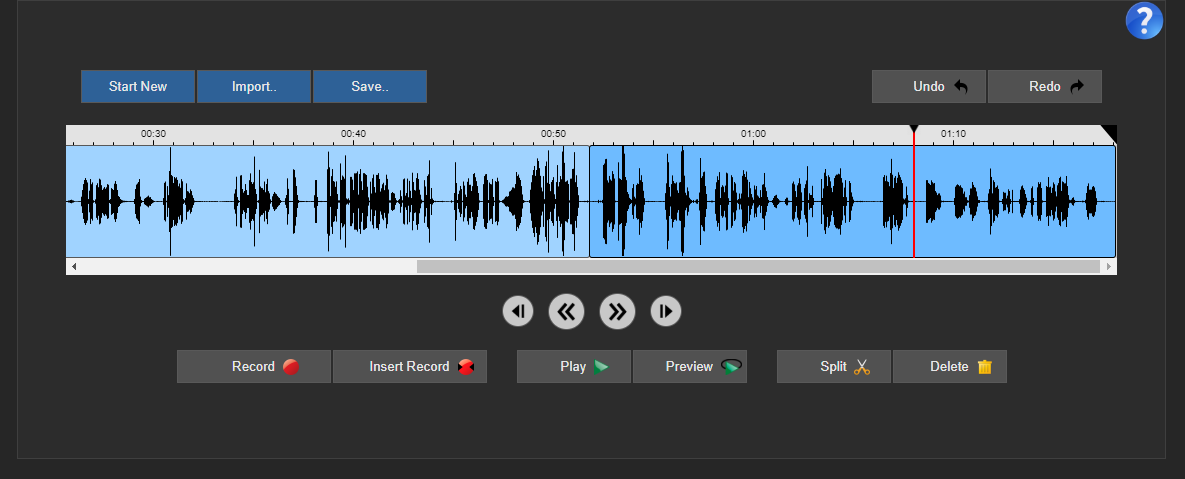
\includegraphics[height=7cm,keepaspectratio]{UI}
  \caption[]{Äänipalautetyökalun käyttöliittymä tietokone-koossa.}
  \label{fig:UI}
\end{figure}

\begin{figure}[h]\centering
  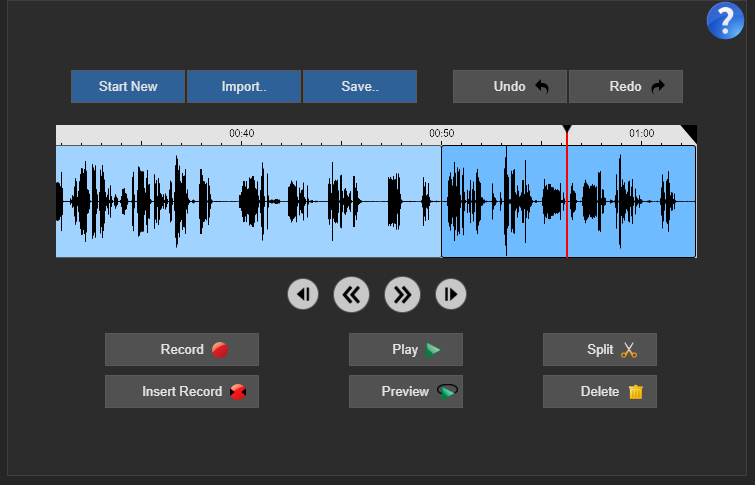
\includegraphics[height=7cm,keepaspectratio]{UI_tablet}
  \caption[]{Äänipalautetyökalun käyttöliittymä tabletti-koossa}
  \label{fig:UI_tablet}
\end{figure}

\begin{figure}[h]\centering
  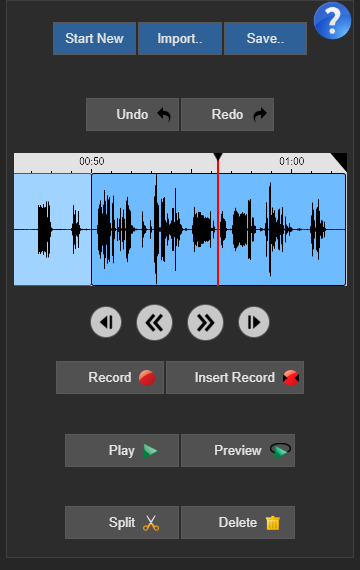
\includegraphics[height=7cm,keepaspectratio]{UI_mobile}
  \caption[]{Äänipalautetyökalun käyttöliittymä mobiili-koossa}
  \label{fig:UI_mobile}
\end{figure}

\section{Perustoiminnot}

Äänipalautetyökalussa on kuusi perustoimintoa, jotka ovat toiminnoista oleellisimpia äänitteiden nauhoittamisen, toistamisen ja editoinnin kannalta. Tässä luvussa käsitellään mitä mikäkin perustoiminto tekee ja perustellaan miksi työkalussa on päädytty juuri kyseisiin toiminnallisuuksiin. Päätöksiin vaikuttavat käytettävyysperiaatteet, suunnittelussa mukana olleiden näkemykset ja aiemmat kokemukset sekä tutkimuksen evaluointi-iteraatiot.


\subsection{Record}

Record-toiminto aloittaa äänipalautteen nauhoittamisen siihen kohtaan äänileikenäkymää, missä äänileikekursori sijaitsee nauhoituksen aloitushetkellä. Jos nauhoitus tapahtuu toisten äänileikkeiden päälle, niin uusi äänileike korvaa alle jääneet äänileikkeet. Nauhoitettava äänileike levenee nauhoituksen edetessä, ja äänileikekursoria liikutetaan äänileikkeen mukana. Kun äänileikekursori saavuttaa äänileikenäkymän oikean reunan, se pysähtyy ja äänileike jatkaa levenemistään. Tällöin nauhoituksen edetessä äänileikenäkymää vieritetään levenevän äänileikkeen oikean reunan mukana.

\subsection{Insert Record}

Insert Record -toiminto nauhoittaa uuden äänileikkeen jo olemassa olevan äänileikkeen väliin. Toiminto katkaisee aluksi sen äänileikkeen kahteen osaan, jonka väliin ollaan nauhoittamassa uutta äänileikettä. Sitten katkaisukohtaan aletaan nauhoittamaan uutta äänileikettä, ja nauhoituksen edetessä oikealla puolella olevia äänileikkeitä kuljetetaan uuden äänileikkeen mukana. 

Kuten tavallisessa nauhoituksessa, niin myös väliinnauhoituksessa äänileikkeen ja kursorin saavuttaessa äänilekenäkymän oikean reunan, kursorin eteneminen pysäytetään ja äänileikenäkymää vierietetään uuden äänileikkeen oikean reunan mukaisesti.

\subsection{Play}

Play-toiminto aloittaa äänipalautteen toistamisen siitä kohdasta missä äänileikekursori sijaitsee toiston aloitushetkellä. Äänileikekursoria liikutetaan toiston edetessä eri tavoin riippuen sen sijainnista ja sitä ympäröivistä äänileikkeistä. Kursoria liikutetaan äänileikenäkymässä oikealle päin siihen asti, kunnes se melkein saavuttaa äänileikenäkymän oikean reunan. Kursorin ja äänileikenäkymän oikean reunan välille jätetään pieni väli, jotta toiston edetessä nähdään pieni tulossa oleva pätkä toistettavasta äänileikkeestä. Jos äänileikenäkymässä on vieritysvaraa oikealle päin, eli toisin sanoen kursoria seuraavia äänileikkeitä, niin äänileikekursori pysähtyy paikalleen ja äänileikenäkymää vieritetään oikealle päin. Kun äänileikenäkymä saavuttaa sen pisteen, ettei vieritettävää enää ole, niin se luonnollisesti pysähtyy ja äänileikekursoria liikutetaan oikealle, kunnes äänileikenäkymän oikea reuna saavutetaan.
 

\subsection{Preview}

Toimii lähes samalla tavalla kuin Play-toiminto, eli aloittaa äänipalautteen toiston siitä kohdasta, missä äänileikekursori toiston aloitushetkellä sijaitsee. Ainut poikkeavuus tavalliseen toistoon on se, että toiston loputtua äänileikekursori palautetaan toiston aloituskohtaan. 

\subsection{Split}

Split-toiminto katkaisee äänileikkeen kahtia siitä kohasta, missä äänileikekursori sillä hetkellä sijaitsee. Katkaisun jälkeen äänileikekursoria siirretään yhden pikselin verran vasemmalle, jolloin se vasemmanpuoleisen katkotun äänileikkeen päällä. Tällöin vasemmanpuoleinen katkaistu äänileike myös asetetaan valinnan alaiseksi, eli se korostetaan tummemmalla värillä.

\subsection{Delete}

Delete-toiminto poistaa halutun äänileikkeen äänileikenäkymästä. Äänileikkeistä poistetaan se, mikä on äänileikekursorin alla poiston aloitushetkellä. Poistettavaa äänileikettä ympäröivät äänileikkeet siirretään yhteen poiston tapahduttua ja äänileikekursori siirretään näiden äänileikkeiden liittymiskohtaan.

\section{Erikoistoiminnot}

Erikoistoimintojen toteutus jouduttiin aikataulusyistä rajaamaan tutkimuksen ulkopuolelle. Toiminnallisuudet on kuitenkin osittain suunniteltu ja evaluoinnin suoirittavilla koehenkilöillä on mahdollisuus ilmaista ajatuksiaan erikoistoimintoihin liittyen arviointilomakkeella. 

\subsection{Start New}

Start New -toiminto palauttaa äänipalautetyökalun alkutilaan uuden äänipalautteen työstämistä varten. Äänileikenäkymä siis tyhjennetään äänileikkeistä ja Undo - Redo -historia tyhjennetään. Uudelleenaloittaminen varmistetaan käyttäjältä ponnahdusikkunan avulla.

\subsection{Import}

Import-toiminnon avulla käyttäjä pystyy tuomaan jo nauhoitetun äänipalautteen omasta tiedostojärjestelmästään äänipalautetyökaluun työstöä varten. Tuotu äänitiedosto asetetaan äänileikenäkymään uutena äänileikkeenä. 

\subsection{Save}

Save-toiminnolla työstetty äänipalaute saadaan tallennettua, joko äänitiedostona tai projektitiedostona, jolloin se voidaan avata äänipalautetyökalussa uudestaan.

%

\chapter{Evaluoinnin tulokset}

Tässä luvussa esitetään äänipalautetyökalun evaluoinnin tulokset, ja niiden pohjalta laaditut jatkotoimenpiteet. Tutkimus sisälti kaksi iteraatiota, joista molemmat päättyivät työkalun evaluointiin. Ensimmäisen evaluaation suorittivat tutkielman ohjaajat Anneli Heimbürger ja Ville Isomöttönen (H1-H2). Toiseen iteraatioon osallistui heidän lisäksi opettajat Paavo Nieminen ja Harri Keto (H3-H4).  Tarkemmat tiedot evaluoinnin suorittamisesta on esitetty luvussa X, ja linkki evaluointien kyselylomakkeeseen löytyy tutkielman liitteet-osiosta.

\section{Ensimmäinen iteraatio}

\subsection{tulokset}

Molemmat ensimmäisen iteraation suorittaneista koehenkilöistä kokivat, että äänipalautetyökalu kokonaisuudessaan palveli tarkoitustaan, eli äänipalautteen antamista, mutta työkalun käytön aikana ilmeni kuitenkin  ongelmia ja ohjelmointivirheitä. Voidaan siis todeta, että tavoitteisiin liittyvistä evaluointikriteereistä tehokkuus, eli tarkoituksenmukaisuus, on saavutettu, mutta työkalussa on vielä parannettavaa toista iteraatiota varten. Tämä oli odotettavaa, sillä ensimmäisen iteraation tärkeimpänä tehtävänä oli selvittää, onko äänipalautetyökalun toteutus menossa oikeaan suuntaan, ja lyötää käyttöä eniten hankaloittavat ohjelmointivirheet.

Molemmat ensimmäisen iteraation koehenkilöistä kokivat, että äänipalautetyökalu helpottaisi äänipalautteen antamista entuudestaan jollain tapaa. Toinen koehenkilöistä perusteli tätä käyttöliittymän joustavuudella, ja toinen insert-record -toiminnon tarjoamalla lisäarvolla. Molempien koehenkilöiden suhtautuminen äänipalautteen antamiseen oli jo entuudestaan hyvä, joten äänipalautetyökalun koekäytöllä ei ollut siihen vaikutusta.

Molemmilla koehenkilöistä oli muutamia huomioita liittyen työkalun perustoimintoihin. Toinen koehenkilöistä ehdotti, että molemmat nauhoitustoiminnot, record ja insert record, voisivat nauhoituksen jälkeen palata nauhoitetun äänileikkeen alkuun, jotta lisäyksen kuuntelu olisi mahdollisimman vaivatonta. Lisäyksenä hän mainitsi, että tämä voisi olla optio-tyyppinen valinta, eli käyttäjä voisi itse valita siirretäänkö äänileikekursori nauhoituksen jälkeen äänileikkeen alkuun.

Toiselle koehenkilöistä jäi testauksessa epäselväksi kuinka split-toiminto toimii, sillä hän huomannut äänipalautetyökalun oikeassa yläkulmassa sijaitsevaa kysymysmerkki-ikonia, jossa työkalun perustoiminnot on selitettynä. Evaluointilomakkeella on maininta ohjeikkunan olemassaolosta, mutta lomakkeella on suuri määrä muuta informaatiota, joten on ymmärrettävää, että koehenkilöltä jää jokin seikka huomaamatta. Hän tarkoituksenaan oli poistaa split-toiminnolla äänileikkeen lopusta pätkä, joten hän katkaisi toiminnolla äänileikkeen haluamastaan kohdasta. Äänileikkeen katkaisun jälkeen äänileikkeistä edellinen korostetaan valituksi, joten delete-toimintoa painettuaan äänileikkeistä vasemmanpuoleinen poistetaan jälkimmäisen sijasta. Split - ja Delete-toimintojen välissä olisi siis tarvinnut siirtää äänileikekursori jälkimmäisen äänileikkeen päälle, jotta poistaminen olisi kohdistunut siihen.

Toinen koehenkilöistä kirjasi vapaamuotoiseen palautteeseen maininnan siitä, että käytti testauksessa firefox-selainta, sekä arvioi testauksessa ITKS452 Requirement Engineering -kurssin parityötä. Hän koki erityisesti insert-record -toiminnon hyvänä ominaisuutena, sekä uskoo, että myös split-toiminto on hyödyllinen, kunhan oppii sen ja delete-toiminnon välisen suhteen. Hän suoritti testauksen tietokoneella.

Toinen koehenkilöistä kirjasi vapaamuotoiseen palautteeseen huomioita ohjelmistoon liittyvistä bugeista. Hän testasi artefaktia iphone 6 -mobiililaitteella Mozilla firefox - ja Chrome-selaimilla, mutta hyödynti testauksessa apuna myös tietokonetta. Hän koki, että äänipalautetyökalun painikkeet asettuivat ruudun kokoon hyvin, ja että työkalun avustus-ikkunan ohjeistukset olivat selkät. Mobiililaitteella ääniaallon piirtämisessä äänileikkeeseen ilmeni kuitenkin ongelmia, sillä amplitudi piirtyi liian suurena. Tästä johtuen äänileikkeet peittyivät paikoin täysin mustalla värillä, jota käytetään ääniaallon piirtämisessä. Ongelman syytä ei saatu selville, mutta se liittyy todennäköisesti siihen, että kyseessä oli iOS-laite, joilla työkalua ei ole laitteiden ja aikataulun rajallisuudesta johtuen testattu. Yksi syy myös iOS-laitteiden tukemattomuudelle oli se, että iOS:in selain Safari ei vielä tutkimuksen tekohetkellä tue täysin äänen nauhoittamiseen tarvittavia rajapintoja. Arviointilomakkeella on tästä johtuen suositus siihen, että testaus moniililla suoritettaisiin android-laitteella. Viimeinen vapaamuotoisen palautteen huomio oli se, että tietokoneella nauhoituksen ollessa päällä, toisen ikkunan, tässä tapauksessa tekstieditorin, aktivoiminen keskeytti nauhoittamisen.

Evaluointilomakkeen viimeinen osio koski kehitysideoita äänipalautetyökalua koskien. Koehenkilö, joka huomasi tarpeen nauhoitetun äänileikkeen alkuun navigointiin, ehdotti siihen tarkoitukseen jonkinlaista painiketta, kuvaketta tai optio tyyppistä valintaa. Lisäksi hän koki, että navigointi jollain tapaa äänileikenäkymän loppuun saattaisi olla tarpeellista. Kolmas navigointiin liittyvä ehdotus oli se, että valitun äänileikkeen alkuun voitaisiin navigoida esimerkiksi jostain pikanäppäinyhdistelmästä, kuten "SHIFT + NUOLI". Navigointiin liittyi myös sellainen huomio, että mobiililaitteella äänileikenäkymän vierityspalkki voisi olla selkeämmin erottuvissa. Hänen viimeinen kehitysideansa koski erikoistoimintopainikkeiden tekstejä. "New File":n sijaan selkeämpi vaihtoehto voisi olla "Start New", ja "Export":in sijaan käyttäjälle intuitiivisempi voisi olla "Save".

\subsection{jatkotoimenpiteet}

Ensimmäisen evaluoinnin keskeisin tulos oli se, että työkalun voidaan sanoa palvelevan tarkoitustaan, ja että käyttöliittymä on selkeä ja ymmärrettävä, muutamia huomioita ja bugeja lukuunottamatta. Merkittävin käytettävyyteen negatiivisesti vaikuttava tekijä oli navigoinnin puutteellisuus, sillä äänileikenäkymässä navigoiminen vaati sen, että äänileikenäkymän vierityspalkkia jouduttiin vierittämään siihen asti, kunnes haluttu kohta löydettiin. Navigoinnista maininneen koehenkilön ehdotukset koskivat lähinnä tietyn äänileikkeen alkuun, ja äänileikenäkymän loppuun navigointia, mutta navigointi voitaisiin toteuttaa näiden spesifien toimintojen sijaan siten, että äänileikenäkymässä pystytään navigoimaan sekä eteen- että taaksepäin äänileike kerrallaan tai suoraan ääripäästä toiseen. Koehenkilö pohti myös sellaista vaihtoehtoa, että käyttäjällä olisi mahdollisuus valita, siirretäänkö äänileikenäkymän kursori nauhoituksen jälkeen kyseisen äänileikkeen alkuun, mutta tämä heikentäisi työkalun intuitiivisuutta, eikä tällöin perustoimintojen johdonmukaisuus toteutuisi niin hyvin.

Ratkaisua navigointiin haettiin muista audio-ohjelmistoista, sillä standardien noudattamisessa on aina omat hyötynsä. Koska vastaavanlaisia äänipalautetyökaluja ei ole saatavilla, niin tutkimustyö kohdistui lähinnä perinteisiin nauhoitustyökaluihin ja musiikkiohjelmistoihin. Useissa audio-ohjelmistoissa navigointi on toteutettu siten, että navigointi on mahdollista tehdä molempiin suuntiin, ja navigointipainikkeita on kahden tyyppisiä: toiset navigoivat ääripäihin, eli alkuun ja loppuun, kun taas toiset navigoivat pienempiä osuuksia jompaan kumpaan suuntaan. Painikkeiden asettelu toisiinsa nähden on myös usein toteutettu siten, että pienempiä osuuksia kelaavat painikkeet ovat sisimpänä, ja niitä ympäröivät ääripäihin kelaavat painikkeet. Navigointipainikkeista palautetta antanut koehenkilö piti myös tätä ratkaisua hyvänä, joten se päätettiin toteuttaa seuraavaa iteraatiota varten. Äänileikkeiden välillä navigointi päätettiin myös mahdollistaa koehenkilön ehdottamalla pikanäppäinyhdistelmällä "SHIFT + NUOLI OIKEALLE TAI VASEMMALLE". Navigaatiotoimintojen suunnitteluratkaisut ja toteutus on tarkemmin käsitelty luvussa X.

Ensimmäisestä evaluoinnista kävi ilmi, että äänipalautetyökalun oikeassa yläkulmassa sijaitseva kysymysmerkki-ikoni oli liian pieni, sillä toinen koehenkilöistä ei sitä testauksen aikana havainnut. Hän olisi kaivannut avustusta Split-toiminnon ymmärtämiseen, mutta se jäi hänelle epäselväksi, sillä avustusikkunan avaava ikoni jäi huomaamatta. Perustoimintoihin harkittiin suunnitteluvaiheessa työkaluvihjeiden käyttöönottoa, joiden ideana on näyttää tekstikentässä sen toiminnon kuvaus lyhyesti, jonka päällä hiiren kursori on tietyllä hetkellä. Niiden toteutuksesta kuitenkin luovuttiin, sillä osaa toiminnoista on vaikeaa kuvailla muutamilla sanoilla, kuten työkaluvihjeillä yleensä on tapana. Tästä johtuen työkaluun toteutettiin erillinen avustusikkuna, jossa työkalun eri toiminnallisuuksien kuvaukset ja pikanäppäimet on esitetty ytimekkäästi. Seuraavaa iteraatiota varten kysymysmerkki-ikonia tulee kuitenkin selvästi suurentaa, jotta käyttäjät huomaisivat sen apua tarvitessaan.

Koehenkilön iOS-laitteella esiintynyttä ääniaaltojen piirtymiseen liittyvää ongelmaa tutkittiin alustavasti, mutta ongelmaa ei saatu toistumaan android-laitteilla. Vaikka bugi vaikuttaa käytettävyyteen negatiivisesti, niin ongelman korjaukseen ei ole järkevää kuluttaa enempää resursseja, sillä evaluoinnin kohteena on prototyyppi, jonka vaatimuksista on jätetty pois tuki iOS:ille, tiettyjen nauhoittamiseen liittyvien rajoitteiden vuoksi. 

Pienemmistä kehitysideoista toteutukseen sisällytettiin erikoistoimintojen painiketekstien muuttaminen koehenkilön ehdottamilla tavoilla. "New File":n siis korvaa "Start New" ja "Export":in "Save". Sama koehenkilö ehdotti myös vieritypalkin vierittimen korostamista esimerkiksi tummemmalla värillä, mikä oli oli erittäin hyvä kehitysidea. Se joduttiin siitä huolimatta jättämään toteutuksen ulkopuolelle, sillä selainten vierityspalkit eivät ole helposti kustomoitavissa vielä tämän tutkimuksen tekohetkellä, ja oman vierityspalkin toteuttaminen vaatisi suurehkoja muutoksia ohjelmiston arkkitehtuuriin, ja aiheuttaisi runsaasti lisätyötä. 

\begin{table}
\centering
\caption{Yhteenveto evaluoinnin huomioista ja jatkotoimenpiteistä}
\begin{tabular}{|l|l|} 
\hline
\textbf{Huomiot}                                                                                                                                                                & \textbf{Jatkotoimenpiteet}                                                                                                                                                                                       \\ 
\hline
\begin{tabular}[c]{@{}l@{}}Kysymysmerkki-ikoni ei ole tarpeeksi \\selkeästi havaittavissa.\end{tabular}                                                                          & \begin{tabular}[c]{@{}l@{}}Korostetaan kysymysmerkki-ikonia \\sen kokoa suurentamalla.\end{tabular}                                                                                                                  \\ 
\hline
\begin{tabular}[c]{@{}l@{}}Navigointi tulisi mahdollistaa \\tietyn äänileikkeen alkuun ja äänileike-\\näkymän loppuun.\end{tabular}                                                 & \begin{tabular}[c]{@{}l@{}}Toteutetaan navigointoiminnot, jotka \\ mahdollistavat äänileikkeiden ja \\ äänileikenäkymän ääripäiden välisen \\navigoinnin sekä eteen- että taaksepäin.\end{tabular}  \\ 
\hline
\begin{tabular}[c]{@{}l@{}}Tietyn äänileikkeen \\alkuun tulisi pystyä navigoimaan \\myös pikanäppäimen avulla.\end{tabular}                                                              & \begin{tabular}[c]{@{}l@{}}Toteutetaan navigointi äänileikkeiden \\välillä pikanäppämellä "CTRL + NUOLI \\VALITTUUN SUUNTAAN".\end{tabular}                                                                                  \\ 
\hline
\begin{tabular}[c]{@{}l@{}}Erikoistoimintojen painiketekstit "New File" \\ja "Export" voidaan korvata intuitiivisemmilla \\vaihtoehdoilla, kuten "Start New"\\ja "Save".\end{tabular} & \begin{tabular}[c]{@{}l@{}}"New File":n korvaa "Start New" ja \\"Export":in korvaa "Save".\end{tabular}                                                                                                          \\
\hline
\begin{tabular}[c]{@{}l@{}}Äänileikkeiden ääniaallot eivät piirry \\oikein koehenkilön iOS-\\laitteella.\end{tabular}                                                            & \begin{tabular}[c]{@{}l@{}}Ei käytetä resursseja ongelman \\selvittämiseen, sillä tuki iOS-laitteille \\on rajattu ulos äänipalautetyökalun \\vaatimuksista.\end{tabular}                                                             \\ 
\hline
\end{tabular}
\end{table}

\section{Toinen iteraatio}

\subsection{Tulokset}

Koehenkilöistä jokainen koki, että äänipalautetyökalu palveli tarkoitustaan, mikä oli tämän tutkimuksen yksi tärkeimmistä tavoitteista. Lisäksi he olivat sitä mieltä, että äänipalautetyökalussa on tiettyjä ominaisuuksia, jotka helpottavat tai nopeuttavat äänipalautteen antamista jollain tapaa. Yksi koehenkilöistä mainitsi, että helpottuminen olisi varmasti havaittavissa siinä vaiheessa, kun työkalun kaikki toiminnot on opeteltu kunnolla. Työkaluun on oppimiskynnyksen minimoimiseksi toteutettu mahdollisimman vähän toiminnallisuuksia, joten siihen ei pitäisi kulua paljoa aikaa. Vaikka työkalu koettiin tarkoituksenmukaiseksi, se ei muuttanut koehenkilöiden suhtautumista äänipalautteen antamiseen, sillä kukin heistä suhtautui siihen jo aluneperin positiivisesti. Kuitenkin koehenkilöt kokivat, että äänipalautetyökalu toisi lisäarvoa äänipalautteenantoon, ja tekisi siitä joustavampaa, sillä äänipalaute voitaisiin antaa laitteesta riippumatta muuallakin kuin työhuoneessa.

Ensimmäisen evaluaation pohjalta lisättyjen navigointipainikkeiden toiminnallisuus ja visuaalisuus koettiin selkeiksi jokaisen koehenkilön toimesta. Yksi koehenkilöistä mainitsi navigoinnin olevan intuitiivista sekä painikkeiden että pikanäppäinyhdistelmien avulla. Hän myös pohti, onko äänileikenäkymän oikeassa yläreunassa näytettävä musta kolmio enää tarpeellinen, sillä navigointi on jo toteutettu työkaluun erillisten painikkeiden avulla. Eräs koehenkilö taas toi esille, että navigointipainikkeet olivat nänelle selkeitä aiemmin käyttämistään työkaluista, ja ne tuntuivat tutuilta ja turvallisilta.

Kuudesta perustoiminnosta neljä koettiin täysin selkeiksi, mutta Preview- ja Split-toimintoihin liittyi tiettyjä huomioita. Yksi koehenkilöistä päätteli aluksi, että Split-toiminto jo itsessään  poistaisi jotain, sillä painikkeen ikonina on sakset, ja tekstinä "Split", joten hän käytti hetken pohtiakseen, kuinka poistokohta merkattaisiin. Kokeiltuaan toimintoa hän kuitenkin oppi, että nimenomaan Split-toiminnon tarkoitus on merkata/katkaista äänileikkeen poistokohdat ja Delete-toiminnolla sitten poistaa tietty äänileike. Sattuneesta syystä, hän pohti, tulisiko termin "Split" sijaan käyttää esim. "Mark":ia tai "Mark split":tiä, mutta oli toiminnon opittuaan tyytyväinen toiminnallisuuteen myös sellaisenaan. Lisäksi hänelle oli aluksi epäselvää, mitä Preview-toiminnosta tapahtuu, mutta kokeiltuaan sitä, hän hoksasi sen, ja löyti toiminnon kuvauksen myöhemmin myös avustus-ikkunasta. Toisen koehenkilön huomio koskien Preview-toimintoa liittyi siihen, että toiminnon ollessa käynnissä painikkeen teksti voisi olla "Pause":n sijaan "Stop", sillä "Pause" useimmissa käyttöyhteyksissä pysähtyy yleensä siihen kohtaan missä kursori sattuu sillä hetkellä olemaan. Kolmas koehenkilö taas pohti, onko Preview-toiminto edes tarpeellinen, sillä kursorin avulla voidaan navigoida helposti tiettyyn kohtaan äänileiikettä ja toistaa se sitten play-toiminnolla. Perustoimintoja koskien, vastauksissa tuli esille myös positiivisia huomioita Insert-Record -toimintoa koskien, mikä koettiin tehokkaaksi toiminnoksi. Eräs koehenkilö oli sitä mieltä, että kyseinen toiminto mahdollistaa äänitteen väliin-nauhoittamisen helpommin, kuin mikään hänen aiemmin kokeilemansa audio-ohjelmisto.

Molemmat ensimmäiseen evaluointiin osallistunutta koehenkilöä kokivat, että käyttöliittymä on selkeytynyt ja parantunut entisestään. Tätä he perustelivat muunmuassa sillä, että kysymysmerkki-ikonia oli suurempi, jolloin avustus-ikkuna oli helpommin löydettävissä, sekä sillä, että navigointitoiminnot helpottivat äänileikenäkymässä navigointia. Toinen ensimmäistä kertaa äänipalautetyökalua evaluoivista koehenkilöistä koki, että äänipalautetyökalu on sopivan yksinkertainen, mikä on positiivista. Eräs koehenkilöistä ilmaisi, että vastaavanlaiselle työkalulle olisi tarvetta, ja siitä voisi kehkeytyä tulevaisuudessa myös natiivisovellus mobiililaitteille. Tämä samainen henkilö testasi työkalua ensimmäisessä iteraatiossa iphone-laitteella, mutta siinä ilmaantuneiden teknisten ongelmien vuoksi hyödynti toisessa iteraatiossa selaimen mobiililaite-emulointia, ja koki työkalun toimivaksi myös mobiilikoossa, siitäkin huolimatta, että äänen kanssa ilmaantui jonkinlaisia ongelmia. Myös eräällä toisella koehenkilöllä oli äänentoistoon liittyviä ongelmia, jotka ilmaantuivat siten, että kunkin äänileikkeen lopusta jäi toistamatta noin sekunnin verran äänitettä.

Kolme koehenkilöistä otti kantaa kyselylomakkeella mainittuun ideatason perustoimintoon, joka mahdollistaisi tekstin lisäämisen tiettyyn kohtaan äänileikettä. Yksi heistä oli sitä mieltä, että se olisi hyvä idea, sillä sen avulla voitaisiin korostaa palautteen keskeisiä asioita, ja tarkentaa niitä sitten puheella. Toinen taas pohti, että se saattaisi olla erittäin toimiva lisäominaisuus, jollaiseen hän ei ole törmännyt muiden audio-ohjelmistojen kohdalla.  Kolmas koehenkilöistä ei pitänyt tekstitoiminnallisuutta itselleen tärkeänä, sillä hän hyödyntää äänipalautetta lähinnä tekstimuotoisen palautteen lisänä kommenttiraita-tyyppisesti. Hän kuitenki pohti, että äänileikkeiden upottaminen tehtävän tiettyihin kohtiin voisi olla hyvä lisäominaisuus, mutta koska kyseessä voisi olla pdf-tiedosto, kuva, lähdekoodi, tai usean tiedoston rypäs sen toteuttamiseen liittyisi runsaasti haasteita.

Toisessa evaluoinnissa tuli esille myös muita kehitysideoita. Yksi koehenkilöistä otti kantaa palautteen tallentamiseen ja oli sitä mieltä, että tallentaminen kannattaisi hänen mielestään tehdä mahdollisimman yksinkertaisesti, esimerkiksi käyttöjärjestelmän perustallennusta hyödyntäen, ja että tiedostojen nimeämiseen voisi olla jokin tuki, joka ehdottaisi esimerkiksi etuliitettä tai kokonaisuuteen liittyvää tunnistetta. Toinen koehenkilö taas oli sitä mieltä, että työkalu olisi parhaimmillaan integroituna oppimisympäristöön, johon tehtäväkin on palautettu, jolloin sekä palaute että tehtävä olisivat samassa ympäristössä, ja erillisen työkalun aiheuttamaa säädöltä vältyttäisiin. Hän oli myös sitä mieltä, että äänipalautetyökalun hyödyntämistä tulisi tutkia erityisesti äänipalautteenannon täysmittaisessa työnkulussa, jossa otettaisiin huomioon kaikki vaiheet nauhoituksesta jakamiseen ja vastaanottamiseen. Tähän hän ehdotti menetelmäksi esimerkiksi opettajien ja oppilaiden suorittamaa käyttäjätestausta, jolla voitaisiin saada selville erilaisia tarpeita äänipalautteen antamiseen ja vastaanottamiseen liittyen.

\subsection{Jatkotoimenpiteet}

Kahden evaluoinnin perusteella voidaan sanoa että äänipalautetyökalu on tarkoituksenmukainen, yksinkertainen ja helppokäyttöinen. Evaluoinneissa ilmeni kuitenkin useita hyviä huomioita ja ideoita työkalun eri osa-alueita koskien, joista osa pystytään ja on pystytty toteuttamaan työkaluun. Osa huomioista ja ideoista joudutaan kuitenkin jättämään ajatuksen tasolle, sillä tämä suunnittelututkimus on rajattu ainoastaan kahteen iteraatioon. Siitä huolimatta ne ovat tärkeitä, varsinkin, jos äänipalautetyökaluun liittyvää tutkimusta aiotaan jatkaa tulevaisuudessa tai siitä päätetään toteuttaa kokoversio. Myös evaluoinneissa esille tulleet bugit on hyvä kirjata ylös mahdollisia jatkotoimenpiteitä silmällä pitäen.

Merkittävimpänä huomiona työkalun käytettävyyden kannalta voidaan pitää Split-toiminnon ymmärrettävyyttä.

%

\chapter{Pohdinta}

-Kahden evaluoinnin perusteella äänipalautetyökalun voidaan sanoa olevan tarkoituksenmukainen, yksinkertainen ja helppokäyttöinen, joten tutkimuksen tavoitteet artefaktin suhteen ovat toteutuneet hyvin.

- toteutettiin äänipalautetyökalu-prototyyppi
- tutkimusmetodi suunnittelututkimus, jonka tarkoituksena ratkaista reaalimaailman ongelmia innovatiivisten artefaktien avulla
- Artefakti kehitettiin ja evaluoitiin kahdessa iteraatiossa
- Evaluointien tavoitteet: bugien löytäminen, toteutuuko tarkoituksenmukaisuus, onko helppokäyttöinen, millaisia kehitysideoita, sekä oleellisimpana tutkimuskysymyksiin vastaaminen.
- Tulosten pohjalta pyritään vastaamaan seuraaviin tutkimuskysymyksiin: 1. voidaanko äänipalautteen antamista helpottaa siihen suunnatun työkalun avulla? 2. Muuttiko äänipalautetyökalun käyttö suhtautumista äänipalautteen antamiseen?

- Toteutettiin prototyyyppi, jolla äänipalautteen nauhoittaminen ja editointi onnistuisi mahdollisimman helposti.
- Tutkimuksissa todettu, että äänipalautteen antamiseen liittyy teknisiä vaatimuksia, ja oppimiskynnystä.
- Parissa tutkimuksessa tulee esille, että opettajien mielestä on helpompi vain aloittaa äänipalaute virheen tullessa uudestaan alusta, kuin editoida sitä, mikä osoittaa sen, että sitä pidetään työläänä tai siihen suhtaudutaan huonosti (oppimiskynnys).
- Työkalu toteutettiin web-pohjaisena, jotta sitä voitaisiin käyttää eri laitteilla ja alustoilla
- Tavoitteena oli toteuttaa mahdollisimman helppokäyttöinen äänipalautetyökalu
	- mahd. vähän toiminnallisuuksia
	- responsiivisuus
	- Tutut jutut muista audio-ohjelmistoista (äänileikenäkymä, jotkut perustoiminnot, undo, help)
	- Myös innovatiivisia toiminnallisuuksia (insert-record, äänileikkeiden autom. sijoittelu)
- Suunnittelussa ja heuristisessa arvioinnissa hyödynnettiin Gestaltin ja Nielsenin heuristiikkoja
- Käyttöliittymä suunniteltiin mahdollisimman yksinkertaiseksi. Käytettävyydellä ja ymmärrettävyydellä prototyypin testaamisessa suurempi merkitys kuin estetiikalla.
- Tutkimuksen laajuuden ja aikataulurajoitteiden takia tietyt toiminnallisuudet jouduttiin jättämään ulkopuolelle. (Palautteen tallentaminen tiedostoksi ja sen jakaminen)

- 
- Evaluoidaan prototyyppiä, simuloidusti autenttisessa tilanteessa, joka otettava huomioon.
- Ensimmäisen evaluaation pohjalta työkaluun tehtiin lähinnä pienempiä parannuksia (helpin isontaminen), mutta isompana ominaisuutena lisättiin navigaatiotoiminnot.
- Evaluointien tulosten perusteella voidaan sanoa, että äänipalautetyökalu palvelee tarkoitustaan eli on tarkoituksenmukainen, mikä oli yksi oleellisimmista evaluointikriteereistä.
- Kenttätestauksissa ilmeni joitakin bugeja liittyen mm. ääneen, ääniaallon piirtymiseen, ja muutamia pikkubugeja
- Vaikka oli tiettyjä ongelmia, tulosten perusteella äänipalautetyökalu-prototyypissä tiettyjä ominaisuuksia, jotka helpottavat äänipalautteen antamista verrattuna esim. audacityyn tai muuhun erilliseen audio-ohjelmistoon verrattuna. 
	- insert-recordin tuoma lisäarvo
	- joustava (eri laitteilla ja alustoilla, voidaan käyttää esim. kotisohvalta mobiililla)
	- sisältää vähän ominaisuuksia, toisin kuin useimmat muut audio-ohjelmistot, mutta kuitenkin tarpeeksi samanlainen kuin muut audio-ohjelmistot, joten ei niin suurta oppimiskynnystä, jos jo kokemusta muista.
	- Äänipalautteen antamisen kannalta oleellisimmat ominaisuudet toteutettu web-käyttöliittymään
	- Jos jakaminen olisi toteutettuna työkaluun suoraan, vähentäis säätöä erillisen aduio-ohjelmiston kanssa (esim. audiotiedostojen exporttaamisen säädöt audacityssä)
	- Olisi paras integroituna oppimisympäristöön.
- Jokaisen opettajan suhtautuminen äänipalautteen antamiseen oli jo entuudestaan positiivinen, joten työkalun käytöllä ei ollut vaikutusta siihen.

- Tässä tutkielmassa käsiteltiin aikataulusyistä ainoastaan äänipalautteen nauhoittamista ja editointia, ja tulosten pohjalta voidaan sanoa äänipalautetyökalun tuovan lisäarvoa niihin.
- Yksi potentiaalinen jatkotutkimuksen aihe olisi laajentaa esim. kyseistä prototyyppiä suunnittelututkimuksen menetelmin sellaiseksi, että palautteen jakaminen olisi mahdollisimman vaivatonta sekä opettajille että oppilaille.
- Tutkimuskysymys äänipalautteeseen suhtautumisesta ei ollut tässä tutkimuksessa oleellinen, sillä kaikilla oli jo positiivinen suhtautuminen (toisaalta suhtautuminen ei muuttunut huonompaan suuntaan, mikä on hyvä). Voitaisiin testauttaa protoa sellaisilla, joilla on jostain syystä negatiivinen suhtautuminen äänipalautteen antamiseen.
- Lisäksi kuten yksi palautteenantajista ilmaisi, niin integrointi oppimisympäristöön tai muuhun vastaavan voisi olla erittäin hyvä ratkaisu, mutta aihe vaatisi perehetymistä.
- Kirjallisuudessa tulee esille, että palautteen jakaminen on työläs osa äänipalautteenantoa, joten jakamisen toteuttaminen helpoksi voisi olla ajankäytön kannalta merkittävä säästö.
- Tutkimuksessa tulisi myös selvittää tarkemmin millä palvelimella työkalua kannattaisi hostata, ja mitä palveluita voitaisiin hyödyntää äänitiedostojen jakamisessa siten, että kuluja ei olisi, tai että ne olisivat minimaaliset. Onko tämä edes mahdollista?

- Yhteenvetona äänipalautteen antamiseen suunnitellun työkalun avulla voidaan helpottaa sen antamista, mutta epäselväksi jäi, voidaanko sen avulla muuttaa opettajien suhtautumista sen antamiseen, sillä heillä oli jo entuudestaan positiivinen suhtautuminen siihen.
- Tutkimuksen voidaan katsoa onnistuneen hyvin, sillä prototyypin kehittämisen ja evaluointien yhteydessä löydettiin sellaisia innovatiivisia ratkaisuja, jotka toisivat kokoversion tapauksessa lisäarvoa äänipalautteen antamiseen (insert-record, minimimäärä toimintoja, monialustaisuus).

%

\printbibliography

\appendix
\section{Ensimmäisen iteraation kyselylomake}

bla bla.

\end{document}
